\PassOptionsToPackage{dvipsnames}{xcolor}
\documentclass[
 %reprint,
  twocolumn,
 %superscriptaddress,
 %groupedaddress,
 %unsortedaddress,
 %runinaddress,
 %frontmatterverbose,
 % preprint,
 showpacs,
 showkeys,
 preprintnumbers,
 %nofootinbib,
 %nobibnotes,
 %bibnotes,
 amsmath,amssymb,
 aps,
 prl,
 %  pra,
 % prb,
 % rmp,
 %prstab,
 %prstper,
  longbibliography,
 floatfix,
 %lengthcheck,
 ]{revtex4-2}

%\usepackage{cdmtcs-pdf}

\usepackage{mathptmx}% http://ctan.org/pkg/mathptmx

\usepackage{amssymb,amsthm,amsmath}

\usepackage{tikz}
\usetikzlibrary{calc,shapes.geometric}
\usepackage {pgfplots}
\pgfplotsset {compat=1.8}
\usepackage{graphicx}% Include figure files
%\usepackage{url}

\usepackage{xcolor}


\usepackage{hyperref}
\hypersetup{
    colorlinks,
    linkcolor={blue},
    citecolor={red!75!black},
    urlcolor={blue}
}

\usepackage{mathbbol}

\usepackage{multirow}


\newcommand\myotimes{ }

\begin{document}


\title{Converting nonlocality into contextuality}



\author{Karl Svozil}
\email{karl.svozil@tuwien.ac.at}
\homepage{http://tph.tuwien.ac.at/~svozil}

\affiliation{Institute for Theoretical Physics,
TU Wien,
Wiedner Hauptstrasse 8-10/136,
1040 Vienna,  Austria}



\date{\today}

\begin{abstract}
Diagonalization of matrix pencils provide a uniform technique to transcribe operator-valued violations of Boole's `conditions of possible experience' involving multipartite correlations into contextuality. They also provide structural analysis of the contexts involved, and thereby suggest compact forms of deviations of quantized systems from classical predictions.
\end{abstract}

%\pacs{03.65.Aa, 03.65.Ta, 03.65.Ud, 03.67.-a}
\keywords{contextuality, two-valued states, quantum states, matrix pencil}
%\preprint{CDMTCS preprint nr. x}

\maketitle


\section{Matrix pencils}

In heuristic terms, `quantum contextuality' encompasses any aspect that contradicts classical predictions, with `strong' types of contextuality entailing complete contradictions relative to classical expectations.
In what follows we shall concentrate on `strong quantum contextuality' rendered by operator-valued arguments exhibiting nonlocality.
While the inverse problem---converting contextuality into nonlocality~\cite{cabello2020converting}---can be of empirical importance,
the solution of the former task can identify the particular type of contextuality exhibited.

From a structural standpoint---that is, in terms of the quantum logical algebraic relations of the associated propositions---operator-valued arguments may be closely related,
although they may formally appear to be very different. For instance, as observed by Cabello~\cite{cabello-96,Cabello-2013-Hardylike}, Hardy's theorem \cite{Hardy-92,Hardy-93} can,
in quantum logical terms, be transcribed as a true-implies-false arrangement (in graph theoretical terms, a gadget) of observables~\cite{2018-minimalYIYS,svozil-2020-hardy}.
However, as we shall see in comparing Kochen-Specker (KS) and Greenberger-Horne-Zeilinger (GHZ) arguments, there need not be such a close relationship.

The  algorithmic  and thus constructive
analysis of a transcription process for cases of operator-value arguments demonstrating nonclassical behavior is based on the proper spectral decomposition of the operators involved.
Mutually commuting normal operators (such as Hermitian or unitary operators that commute with their respective adjoints)
 $A_1, \ldots, A_l$ share common projection operators.
However, if their spectra are degenerate we need to find an orthonormal basis in which every single one of this collection of mutually commuting operators is diagonal.
Although in principle well-known~\cite[Section 1.3]{Horn-Johnson-MatrixAnalysis}, the standard procedure via block diagonalization can be rather involved~\cite{Nordgren2020Jun}.
Alternatively, we can diagonalize the matrix pencil:
\begin{equation}
P = \sum_{i=1}^{l} a_i A_i,
\label{2024-convert-matrixpencil}
\end{equation}
where $a_i$ are scalars (for our purposes, real numbers).
As $P$ commutes with $A_1, \ldots, A_l$, they share a common set of projection operators.
Moreover, since the scalar parameters $a_i$ can be adjusted, and in particular, can be identified with Kronecker delta functions $\delta_{ij}$,
and as $P$ commutes with each operator $A_j$ for $1 \le j \le l$, $P$ and $A_j$ share a common set of projection operators.

Equipped with these techniques, any collection of commeasurable multipartite observables corresponding
to mutually commuting operators can be transcribed into
%vectors $|e_i\rangle$ corresponding to the
projection operators
%$E_i = |e_i\rangle \langle e_i|$
in the spectrum of the operators of these observables.
If these operators render a maximal resolution, the respective vectors correspond to an orthonormal basis called a context with respect to $A_1, \ldots, A_l$.
The merging or pasting of possibly intertwining contexts then generates a quantum logic which can be
analyzed to identify and characterize the contextual (nonclassical) predictions and features.

%The matrix pencil of $A_1, \ldots, A_l$ yields a maximal resolution (which not necessarily is unique if $A_1, \ldots, A_l$ is not sufficiently resolving)
%in terms of common eigenvectors.
%The orthogonal projection operators corresponding to these eigenvectors
%can be bundled into a single maximal nondegenerate operator $M = \sum_{i=1}^{n} \mu_i E_i$ with $n$ mutually different eigenvalues $\mu_i$ (of multiplicity one),
%which can be conceived as containing the entirety of possible information available through $A_1, \ldots, A_l$,
%which is all that can be known quantum mechanically~\cite{zeil-99}.
%In this formal sense, the collection of observables $A_1, \ldots, A_l$ may be considered to `correspond to a context'.
%This bridges the gap between general operator-valued arguments on the one hand, and quantum logics on the other hand,
%as the latter is based on the identification of propositions with projection operators~\cite{birkhoff-36}.




\begin{table*}[ht]
\caption{\label{2024-convert-matrixpencil-peres} Eigensystems of the matrix pencils of the rows and columns of the PM square~\eqref{2024-convert-PeresSquare}
with normalization factors omitted.
The eigenvectors corresponding to the last row and column are nonseparable and thus entangled, while all others are separable.
This set of 24 vectors includes the 18 vectors of Cabello, Estebaranz and Garc{\'{i}}a-Alcaine~\cite{cabello-96}.
As already noted by Peres~\cite{peres-91},
these six `primary' contexts associated with orthogonal tetrads are disjoint (not intertwined).
In the hypergraph representation depicted in Figure~\ref{2024-convert-f-24-24}(a) they are represented as the `small ovals' on the six edges of the hypergraph.
%This arrangement of contexts is thus not isomorphic to the (biconnected) 18-9 configuration of Cabello, Estebaranz and Garc{\'{i}}a-Alcaine~\cite{cabello-96}.
%The latter matrix pencil yields the Bell basis $\big\{ \vert \Psi_+ \rangle , \vert \Psi_- \rangle , \vert \Phi_+ \rangle  , \vert \Phi_- \rangle \big\}$.
}
\begin{ruledtabular}
\begin{tabular}{ccccccc}
matrix pencils&\multicolumn{4}{c}{eigenvalues}\\
%\hline
&$a - b - c$& $-a + b - c$& $-a - b + c$&   $a + b + c$\\
\hline
$
a \sigma_z  \myotimes   \mathbb{1}_2 + b \mathbb{1}_2 \myotimes   \sigma_z + c \sigma_z  \myotimes   \sigma_z
$ & $
\vert 7 \rangle = \begin{pmatrix}  0, 1, 0, 0\end{pmatrix}^\intercal $ & $
\vert 3 \rangle = \begin{pmatrix}  0, 0, 1, 0\end{pmatrix}^\intercal $ & $
\vert 1 \rangle = \begin{pmatrix}  0, 0, 0, 1\end{pmatrix}^\intercal $ & $
\vert 17 \rangle = \begin{pmatrix}  1, 0, 0, 0\end{pmatrix}^\intercal
$ \\ $
a \mathbb{1}_2 \myotimes   \sigma_x + b \sigma_x  \myotimes   \mathbb{1}_2 + c \sigma_x  \myotimes   \sigma_x
$ & $
\vert 20 \rangle = \begin{pmatrix}  -1, -1, 1, 1\end{pmatrix}^\intercal $ & $
\vert 13 \rangle = \begin{pmatrix}  -1, 1, -1, 1\end{pmatrix}^\intercal $ & $
\vert 11 \rangle = \begin{pmatrix}  1, -1, -1, 1\end{pmatrix}^\intercal $ & $
\vert 24 \rangle = \begin{pmatrix}  1, 1,  1, 1\end{pmatrix}^\intercal
$ \\ $
a \sigma_z  \myotimes   \sigma_x + b \sigma_x  \myotimes   \sigma_z + c \sigma_y  \myotimes   \sigma_y
$ & $
\vert 21 \rangle = \begin{pmatrix}  1, 1, -1, 1\end{pmatrix}^\intercal $ & $
\vert 14 \rangle = \begin{pmatrix}  1, -1, 1, 1\end{pmatrix}^\intercal $ & $
\vert 23 \rangle = \begin{pmatrix}  -1, 1, 1,  1\end{pmatrix}^\intercal $ & $
\vert 10 \rangle = \begin{pmatrix}  -1, -1, -1, 1\end{pmatrix}^\intercal
$ \\ $
a \sigma_z  \myotimes   \mathbb{1}_2 + b \mathbb{1}_2 \myotimes   \sigma_x + c \sigma_z  \myotimes   \sigma_x
$ & $
\vert 12 \rangle = \begin{pmatrix}  -1, 1, 0, 0\end{pmatrix}^\intercal $ & $
\vert 4 \rangle = \begin{pmatrix}  0, 0, 1, 1\end{pmatrix}^\intercal $ & $
\vert 2 \rangle = \begin{pmatrix}  0, 0, -1, 1\end{pmatrix}^\intercal $ & $
\vert 22 \rangle =  \begin{pmatrix}  1, 1, 0, 0\end{pmatrix}^\intercal
$ \\ $
a \mathbb{1}_2 \myotimes   \sigma_z + b \sigma_x  \myotimes   \mathbb{1}_2 + c \sigma_x  \myotimes   \sigma_z
$ & $
\vert 15 \rangle = \begin{pmatrix}  -1, 0, 1, 0\end{pmatrix}^\intercal $ & $
\vert 8 \rangle = \begin{pmatrix}  0, 1, 0, 1\end{pmatrix}^\intercal $ & $
\vert 6 \rangle = \begin{pmatrix}  0, -1, 0, 1\end{pmatrix}^\intercal $ & $
\vert 19 \rangle = \begin{pmatrix}  1, 0, 1, 0\end{pmatrix}^\intercal
$ \\
\hline
&$a - b - c$& $-a + b - c$& $-a - b + c$&   $a + b + c$\\
\hline
$
a \sigma_z  \myotimes   \sigma_z + b \sigma_x  \myotimes   \sigma_x + c \sigma_y  \myotimes   \sigma_y
$ & $
\vert 5 \rangle = \vert \Psi_- \rangle = \begin{pmatrix}  0, 1, -1, 0\end{pmatrix}^\intercal $ & $
\vert 18 \rangle = \vert \Phi_+ \rangle = \begin{pmatrix}  1, 0, 0, 1\end{pmatrix}^\intercal $ & $
\vert 16 \rangle = \vert \Phi_- \rangle = \begin{pmatrix}  1, 0, 0, -1\end{pmatrix}^\intercal $ & $
\vert 9 \rangle = \vert \Psi_+ \rangle = \begin{pmatrix}  0, 1, 1, 0\end{pmatrix}^\intercal
$
\end{tabular}
\end{ruledtabular}
\end{table*}


\section{Matrix pencils of the Peres-Mermin square}

Applying these techniques to the Peres-Mermin (PM) square~\cite{peres111,mermin90b,peres-91,cabello2021contextuality} renders
24 propositions and 24 contexts, henceforth called the 24-24 configuration,
that is the `completion' of the (minimal in four dimensions~\cite{Pavicic-2005}) 18-9 KS configuration comprising 18 vectors in 9 contexts~\cite{cabello-96}.
In more detail, this configuration involves nine dichotomic observables with eigenvalues $\pm 1$ arranged in a $3 \times 3$ PM matrix~\eqref{2024-convert-PeresSquare}.
Its rows and columns are masking six four-element contexts, one per row and column ($\sigma_i \myotimes \sigma_j$ stands for the tensor product of Pauli spin matrices $\sigma_i \otimes \sigma_j$, with similar notation for $\mathbb{1}_2$)
\begin{equation}
\begin{pmatrix}
\sigma_z \myotimes  \mathbb{1}_2 & \mathbb{1}_2 \myotimes  \sigma_z & \sigma_z \myotimes  \sigma_z \\
\mathbb{1}_2 \myotimes  \sigma_x & \sigma_x \myotimes  \mathbb{1}_2 & \sigma_x \myotimes  \sigma_x \\
\sigma_z \myotimes  \sigma_x & \sigma_x \myotimes  \sigma_z & \sigma_y \myotimes  \sigma_y
\end{pmatrix}
.
\label{2024-convert-PeresSquare}
\end{equation}


To explicitly demonstrate the difficulties involved co-diagonalization of commuting degenerate matrices
consider the last row of  the PM square~(\ref{2024-convert-PeresSquare}).
Its operators
$\sigma_z  \myotimes   \sigma_x$, $\sigma_x  \myotimes   \sigma_z$, and $\sigma_y  \myotimes   \sigma_y $ mutually
commute---for instance, $[\sigma_z  \myotimes   \sigma_x,\sigma_y  \myotimes   \sigma_y]=0$.
However, a straightforward calculation of the eigenvectors of $\sigma_z \myotimes  \sigma_x$ yields:
$\begin{pmatrix}
{0, 1, 0, 1}
\end{pmatrix}^\intercal $,
$\begin{pmatrix}
{-1, 0, 1, 0}
\end{pmatrix}^\intercal $,
$\begin{pmatrix}
{0, -1, 0, 1}
\end{pmatrix}^\intercal $, and
$\begin{pmatrix}
{1, 0, 1, 0}
\end{pmatrix}^\intercal $.
None of these eigenvectors are eigenvectors of $\sigma_y \myotimes  \sigma_y$, and vice versa.
This demonstrates the difficulties involved in co-diagonalizing  commuting degenerate matrices.

Nonetheless, the `joint' PM square contexts are revealed as the normalized eigenvectors of the respective matrix pencils~\eqref{2024-convert-matrixpencil}.
Table~\ref{2024-convert-matrixpencil-peres} enumerates those contexts,
provided that the $\sigma$-matrices are encoded in the standard form.
%$
%\sigma ( \theta ,\varphi ) = \sigma_x \sin\theta \cos\varphi  + \sigma_y \sin\theta \sin\varphi  + \sigma_z \cos\theta
%$,
%where $0 \le \theta \le \pi$ is the polar angle in the $x$--$z$-plane
%from the $z$-axis,
%and $0 \le \varphi < 2 \pi$ is the azimuthal angle in the $x$--$y$-plane
%from the $x$-axis,
%with
%$
%\sigma_x =  {\sigma} \left(\frac{\pi}{2},0\right)= \mathrm{antidiag}\begin{pmatrix} 1 , 1  \end{pmatrix}
%$,
%$
%\sigma_y =  {\sigma} \left(\frac{\pi}{2},\frac{\pi}{2}\right)= \mathrm{antidiag}\begin{pmatrix} -i ,   i  \end{pmatrix}
%$,
%and
%$
%\sigma_z =  {\sigma} \left(0,0\right)= \mathrm{diag} \begin{pmatrix} 1 ,  -1   \end{pmatrix}
%$.
%Then the resulting set of 24 vectors contains all 18 vectors enumerated by Cabello, Estebaranz and Garc{\'{i}}a-Alcaine~\cite{cabello-96},
%but the contexts are enumerated differently and need to be reconstructed through orthogonality relations.
%Both the PM square--through the hypothetical existence of  uniform dichotomic, operator based values,
%as well as the KS set of 18 elements in 9 contexts---through the hypothetical existence of  uniform binary two-valued states,
%support parity proofs of nonclassicality.








%`Directing' or `orienting' the 24 different eigenvectors of
%Table~\ref{2024-convert-matrixpencil-peres}  such that their first non-negative entry is positive, and
%subsequently lexicographically ordering them, results in a list enumerated in Table~\ref{2024-convert-matrixpencil-peres-DirectedLexOrdered}.
%
%\begin{table*}[ht]
%\caption{\label{2024-convert-matrixpencil-peres-DirectedLexOrdered}The 24 vectors specifying the binary observables (propositions) of the PM square,
%with normalization factors omitted.}
%\begin{ruledtabular}
%%\begin{center}
%%\resizebox{0.95\textwidth}{!}{
%\begin{tabular}{lllllllll}
%$ \begin{pmatrix}   0, 0, 0, 1 \end{pmatrix}^\intercal  $, &
%$\begin{pmatrix}   0, 0, 1, -1 \end{pmatrix}^\intercal  $, &
%$ \begin{pmatrix}   0, 0, 1,  0 \end{pmatrix}^\intercal  $, &
%$ \begin{pmatrix}   0, 0, 1, 1 \end{pmatrix}^\intercal  $, &
%$ \begin{pmatrix}   0, 1, -1, 0 \end{pmatrix}^\intercal  $,
%\\
%$ \begin{pmatrix}   0, 1, 0, -1 \end{pmatrix}^\intercal  $, &
%$ \begin{pmatrix}   0, 1, 0, 0 \end{pmatrix}^\intercal  $, &
%$ \begin{pmatrix}   0, 1, 0, 1 \end{pmatrix}^\intercal  $, &
%$ \begin{pmatrix}   0, 1, 1,  0 \end{pmatrix}^\intercal  $, &
%$ \begin{pmatrix}   1, -1, -1, -1 \end{pmatrix}^\intercal  $,
%\\
%$ \begin{pmatrix}   1, -1, -1, 1 \end{pmatrix}^\intercal  $, &
%$ \begin{pmatrix}   1, -1, 0, 0 \end{pmatrix}^\intercal  $, &
%$ \begin{pmatrix}   1, -1,  1, -1 \end{pmatrix}^\intercal  $, &
%$ \begin{pmatrix}   1, -1, 1, 1 \end{pmatrix}^\intercal  $, &
%$ \begin{pmatrix}   1, 0, -1, 0 \end{pmatrix}^\intercal  $,
%\\
%$ \begin{pmatrix}   1, 0, 0, -1 \end{pmatrix}^\intercal  $, &
%$ \begin{pmatrix}   1, 0, 0,  0 \end{pmatrix}^\intercal  $, &
%$ \begin{pmatrix}   1, 0, 0, 1 \end{pmatrix}^\intercal  $, &
%$ \begin{pmatrix}   1, 0, 1, 0 \end{pmatrix}^\intercal  $, &
%$ \begin{pmatrix}   1, 1, -1, -1 \end{pmatrix}^\intercal  $,
%\\
%$ \begin{pmatrix}   1, 1, -1, 1 \end{pmatrix}^\intercal  $, &
%$ \begin{pmatrix}  1,   1, 0, 0 \end{pmatrix}^\intercal  $, &
%$ \begin{pmatrix}   1, 1, 1, -1 \end{pmatrix}^\intercal  $, &
%$ \begin{pmatrix}   1, 1, 1, 1 \end{pmatrix}^\intercal  $
%\end{tabular}
%%}
%%\end{center}
%\end{ruledtabular}
%\end{table*}

Analysis of their orthogonality relations yields an adjacency matrix that, in turn,
can be used to construct the respective  (hyper)graph through the intertwining 24 cliques and thus contexts thereof.
As can be expected, there are only four-cliques corresponding to orthonormal bases in four dimensional Hilbert space.
%They are enumerated in Table~\ref{2024-convert-matrixpencil-peres-DirectedLexOrdered-cliques}.
%Indeed, they represent the completed and extended elements and orthogonality relationships of the Cabello, Estebaranz and Garc{\'{i}}a-Alcaine~\cite{cabello-96} set of 18 vector labels in 9 contexts (also depicted in~\cite[Figure 4(c)]{pavicic-2004ksafq}
%and mentioned in~\cite{pavicic-2010nkss}, as well as~\cite[Figure 2]{2010-qchocolate}).
Figure~\ref{2024-convert-f-24-24}(a) depicts the hypergraph representing these intertwining contexts as unbroken smooth lines,
 and the vector labels as elements of these contexts,
as enumerated in Table~\ref{2024-convert-matrixpencil-peres}.
% and~\ref{2024-convert-matrixpencil-peres-DirectedLexOrdered-cliques}.

The 24 rays were already discussed by Peres~\cite{peres-91} as permutations of the vector components of
$\begin{pmatrix}
{1, 0, 0, 0}
\end{pmatrix}^\intercal $,
$\begin{pmatrix}
{1, 1, 0, 0}
\end{pmatrix}^\intercal $,
$\begin{pmatrix}
{1, -1, 0, 0}
\end{pmatrix}^\intercal $,
$\begin{pmatrix}
{1, 1, 1, 1}
\end{pmatrix}^\intercal $,
$\begin{pmatrix}
{1, 1, 1, -1}
\end{pmatrix}^\intercal $, and
$\begin{pmatrix}
{1, 1, -1, -1}
\end{pmatrix}^\intercal $.
The `full' 24-24 configuration was obtained by Pavi\v{c}i\'{c}~\cite{pavicic-2004ksafq} who
reconstructed additional 18 contexts not provided in the original Peres paper~\cite{peres-91} by hand~\cite{pavicic-private-commun-2024}.
Peres' 24-24 configuration is arranged in four-element contexts  associated with four-dimensional Hilbert space, with vector
components drawn from the set $\{-1,0,1\}$, that do not support any two-valued state.
%An early incomplete representation of the Peres configuration~\cite{peres-91} was presented by Tkadlec~\cite[Figure~1]{tkadlec-00}  who mentions  24 elements in 22 contexts.
Pavi\v{c}i\'{c}, Megill and Merlet~\cite[Table~1]{pavicic-2010nkss}
have demonstrated that Peres' 24-24 configuration contains 1,233 sets that do not support any two-valued states.
Among these 1,233 sets are six `irreducible' or `critical' configurations which do not contain any proper subset that does not support two-valued states.
Notably, among these configurations is the previously mentioned 18-9 configuration proposed by Cabello, Estebaranz and Garc{\'{i}}a-Alcaine~\cite{cabello-96}.
Previously, Pavi\v{c}i\'{c}, Merlet, McKay, and Megill~\cite[Section~5(viii)]{pavicic-2005ksw,pavicic-2005csvcorri} had shown that,
among all sets with 24 rays and vector components from the set $\{-1,0,1\}$, and
24 contexts, only one configuration does not
allow any two valued state---and that one is isomorphic to Peres' `full' (including 18 additional contexts)
24-24 configuration enumerated by Pavi\v{c}i\'{c}~\cite{pavicic-2004ksafq}.
This computation had taken one year on a single CPU of a supercomputer~\cite{pavicic-private-commun-2024}.
More recently, Pavi\v{c}i\'{c} and Megill~\cite[Table~1]{Pavii2018} have demonstrated that the vector components from the set $\{-1,0,1\}$
vector-generate a  24-24 set, which contains all smaller KS sets  and is simultaneously isomorphic to the `completed'  24-24 configuration configuration.


We conjecture without providing a formal proof that if a `larger' collection of quantum observables (such as 24-24) contains a `smaller' collection of quantum observables (such as 18-9),
then it inherits the scarcity or total absence of two-valued states of the latter: if the `smaller' set cannot support features related to two-valued states, such as separability of propositions~\cite[Theorem 0]{kochen1},
then intertwining or adding contexts can only impose further constraints, thereby exacerbating the situation by introducing new conditions.



%\begin{table*}[ht]
%\caption{\label{2024-convert-matrixpencil-peres-DirectedLexOrdered-cliques}The 24 cliques or contexts or orthonormal bases or maximal operators
%of the PM square.
%Numbers $1 \le i \le 24$ refer to  the vectors $ \vert i \rangle $ defined in Table~\ref{2024-convert-matrixpencil-peres-DirectedLexOrdered},
%or, equivalently, to the onedimensional orthogonal projection operator $ E_i = (\vert i \rangle \langle i \vert)/ \langle  i \vert i \rangle   $.}
%\begin{ruledtabular}
%\begin{tabular}{cccccc}
%$ C_{ 1 } =       \big\{ 5, 9, 16, 18 \big\}  $, &
%$ C_{ 2 } =       \big\{ 3, 7, 16, 18 \big\}  $, &
%$ C_{ 3 } =       \big\{ 9, 14, 16, 21 \big\}  $, &
%$ C_{ 4 } =       \big\{ 9, 13, 18, 20 \big\}  $, &
%$ C_{ 5 } =       \big\{ 11, 13, 20, 24 \big\}  $, &
%$ C_{ 6 } =       \big\{ 5, 11, 16, 24 \big\}  $,
%\\
%$ C_{ 7 } =       \big\{ 10, 14, 21, 23 \big\}  $, &
%$ C_{ 8 } =       \big\{ 5, 10, 18, 23 \big\}  $, &
%$ C_{ 9 } =       \big\{ 8, 14, 15, 23 \big\}  $, &
%$ C_{ 10 } =      \big\{ 8, 11, 19, 20 \big\}  $, &
%$ C_{ 11 } =      \big\{ 6, 13, 15, 24 \big\}  $, &
%$ C_{ 12 } =      \big\{ 6, 10, 19, 21 \big\}  $,
%\\
%$ C_{ 13 } =      \big\{ 6, 8, 15, 19 \big\}  $, &
%$ C_{ 14 } =      \big\{ 3, 6, 8, 17 \big\}  $, &
%$ C_{ 15 } =      \big\{ 4, 12, 21, 23 \big\}  $, &
%$ C_{ 16 } =      \big\{ 4, 11, 13, 22 \big\}  $, &
%$ C_{ 17 } =      \big\{ 2, 12, 20, 24 \big\}  $, &
%$ C_{ 18 } =      \big\{ 2, 10, 14, 22 \big\}  $,
%\\
%$ C_{ 19 } =      \big\{ 2, 4, 12, 22 \big\}  $, &
%$ C_{ 20 } =      \big\{ 2, 4, 7, 17 \big\}  $, &
%$ C_{ 21 } =     \big\{ 1, 7, 15, 19 \big\}  $, &
%$ C_{ 22 } =      \big\{ 1, 5, 9, 17 \big\}  $, &
%$ C_{ 23 } =      \big\{ 1, 3, 12, 22 \big\}  $, &
%$ C_{ 24 } =      \big\{ 1, 3, 7, 17 \big\}  $
%\end{tabular}
%\end{ruledtabular}
%\end{table*}



\begin{figure*}[ht]
\centering
\begin{tabular}{ccc}
\begin{minipage}{.43\textwidth}
\resizebox{1\textwidth}{!}{
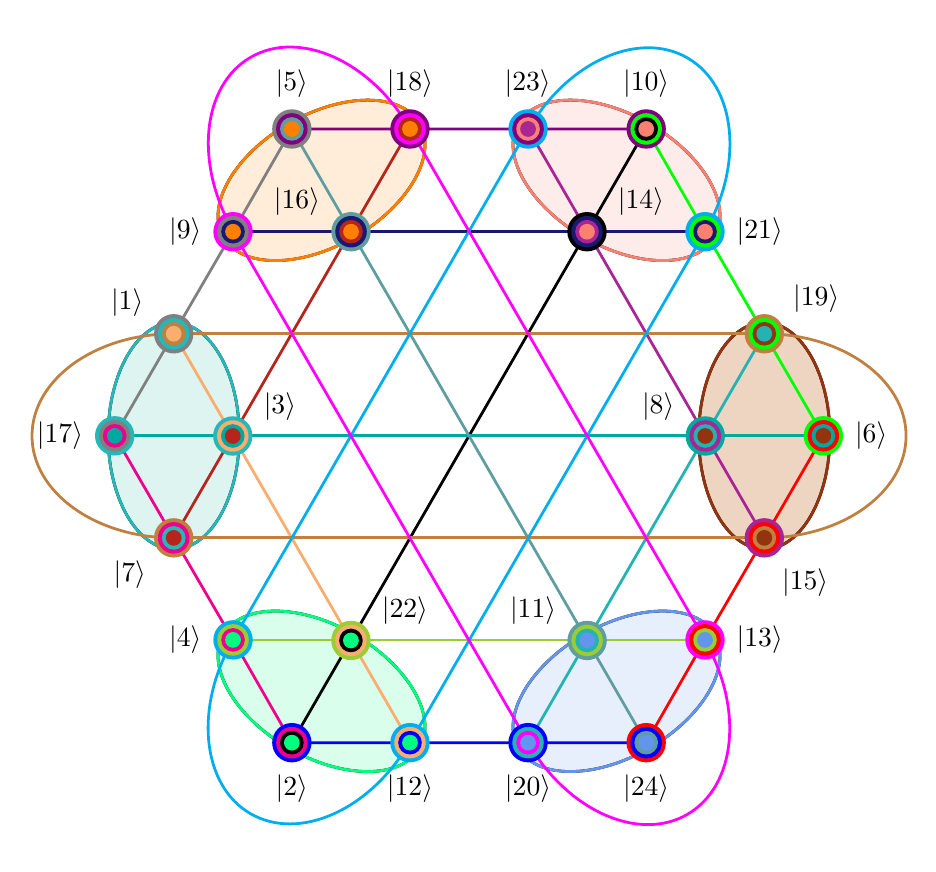
\begin{tikzpicture}  [scale=0.9]
\tikzstyle{every path}=[line width=1pt]   %,label distance=0.6pt
\newdimen\ms
\ms=0.1cm
        %\tikzstyle{c2}=[circle,inner sep=1pt,minimum size=5pt]
        %\tikzstyle{c1}=[circle,inner sep=0pt,minimum size=3pt]
\tikzstyle{c4}=[circle,inner sep={\ms/8},minimum size=5*\ms]
\tikzstyle{c3}=[circle,inner sep={\ms/8},minimum size=4*\ms]
\tikzstyle{c2}=[circle,inner sep={\ms/8},minimum size=3*\ms]
\tikzstyle{c1}=[circle,inner sep={\ms/8},minimum size=2*\ms]



        %%% Define positions of some observables
        \path
              (240:5) coordinate(1)
              (-0.833,-4.33) coordinate(2)
              (0.833,-4.33) coordinate(3)
              (300:5) coordinate(4)
              (3.33,-2.88) coordinate(5)
              (4.167,-1.44) coordinate(6)
              (0:5) coordinate(7)
              (4.167,1.44) coordinate(8)
              (3.33,2.88) coordinate(9)
              (60:5) coordinate(10)
              (0.833,4.33) coordinate(11)
              (-0.833,4.33) coordinate(12)
              (120:5) coordinate(13)
              (-3.33,2.88) coordinate(14)
              (-4.167,1.44) coordinate(15)
              (180:5) coordinate(16)
              (-4.167,-1.44) coordinate(17)
              (-3.33,-2.88) coordinate(18);




        %%% Draw all the context curves

       % small ellipses

\node[ellipse, draw, fill=BlueGreen!15!white, minimum width=1.666cm, minimum height=2.88cm] at (-4.167,0) {};
\node[ellipse, draw, color=BlueGreen, minimum width=1.666cm, minimum height=2.88cm] at (-4.167,0) {};
\node[ellipse, draw, fill=RawSienna!15!white, minimum width=1.666cm, minimum height=2.88cm] at (4.167,0) {};
\node[ellipse, draw, color=RawSienna, minimum width=1.666cm, minimum height=2.88cm] at (4.167,0) {};
\node[ellipse, draw, fill=SpringGreen!15!white, minimum width=1.666cm, minimum height=2.88cm, rotate=60] at (-2.0815,-3.605) {};
\node[ellipse, draw, color=SpringGreen, minimum width=1.666cm, minimum height=2.88cm, rotate=60] at (-2.0815,-3.605) {};
\node[ellipse, draw, fill=Salmon!15!white, minimum width=1.666cm, minimum height=2.88cm, rotate=60] at ( 2.0815, 3.605) {};
\node[ellipse, draw, color=Salmon, minimum width=1.666cm, minimum height=2.88cm, rotate=60] at ( 2.0815, 3.605) {};
\node[ellipse, draw, fill=orange!15!=, minimum width=1.666cm, minimum height=2.88cm, rotate=-60] at (-2.0815, 3.605) {};
\node[ellipse, draw, color=orange, minimum width=1.666cm, minimum height=2.88cm, rotate=-60] at (-2.0815, 3.605) {};
\node[ellipse, draw, fill=CornflowerBlue!15!white, minimum width=1.666cm, minimum height=2.88cm, rotate=-60] at ( 2.0815, -3.605) {};
\node[ellipse, draw, color=CornflowerBlue, minimum width=1.666cm, minimum height=2.88cm, rotate=-60] at ( 2.0815, -3.605) {};


        % outer hexagons

\draw [color=green] (7) -- (8) -- (9)-- (10);
\draw [color=violet] (10) -- (11) -- (12) -- (13);
\draw [color=gray] (13) -- (14) -- (15) -- (16);
\draw [color=magenta] (16) -- (17) -- (18) -- (1);
\draw [color=blue] (1) -- (2) -- (3) -- (4);
\draw [color=red] (4) -- (5) -- (6) -- (7);

        % inner hexagons

\draw [color=Apricot] (2) -- (15);
\draw [color=TealBlue] (3) -- (8);
\draw [color=YellowGreen] (5) -- (18);
\draw [color=MidnightBlue] (9) -- (14);
\draw [color=Mulberry] (11) -- (6);
\draw [color=BrickRed] (12) -- (17);

       % inner diagonals


\draw [color=black] (1) -- (10);
\draw [color=Emerald] (7) -- (16);
\draw [color=CadetBlue] (4) -- (13);





      % outer ovals

        \draw [color=brown] (8) -- (15);
        \draw [color=brown](17) -- (6);
        \draw [color=brown] (8) arc (450:270:2 and 1.44);
        \draw [color=brown] (15) arc (90:270:2 and 1.44);

        \draw [color=cyan] (9) -- (2);
        \draw [color=cyan] (11) -- (18);
        \draw [rotate=240,color=cyan] (9) arc (90:270:2 and 1.44);
        \draw[rotate=60,color=cyan] (18) arc (90:270:2 and 1.44);

        \draw [color=Fuchsia] (12) -- (5);
        \draw [color=Fuchsia] (14) -- (3);
        \draw[rotate=300,color=Fuchsia] (12) arc (90:270:2 and 1.44);
        \draw[rotate=120,color=Fuchsia] (3) arc (90:270:2 and 1.44);




        % Draw the observables themselves
        \draw (1) coordinate[c4,fill=blue,label=270:$\vert 2 \rangle$];
        \draw (1) coordinate[c3,fill=magenta];
        \draw (1) coordinate[c2,fill=black];
        \draw (1) coordinate[c1,fill=SpringGreen];

        \draw (2) coordinate[c4,fill=cyan,label=270:$\vert 12 \rangle$];
        \draw (2) coordinate[c3,fill=Apricot];
        \draw (2) coordinate[c2,fill=blue];
        \draw (2) coordinate[c1,fill=SpringGreen];

        \draw (3) coordinate[c4,fill=blue,label=270:$\vert 20 \rangle$];
        \draw (3) coordinate[c3,fill=TealBlue];
        \draw (3) coordinate[c2,fill=Fuchsia];
        \draw (3) coordinate[c1,fill=CornflowerBlue];

        \draw (4) coordinate[c4,fill=red,label=270:$\vert 24 \rangle$];
        \draw (4) coordinate[c3,fill=blue];
        \draw (4) coordinate[c2,fill=CadetBlue];
        \draw (4) coordinate[c1,fill=CornflowerBlue];

        \draw (5) coordinate[c4,fill=Fuchsia,label=0:$\vert 13 \rangle$];
        \draw (5) coordinate[c3,fill=red];
        \draw (5) coordinate[c2,fill=YellowGreen];
        \draw (5) coordinate[c1,fill=CornflowerBlue];

        \draw (6) coordinate[c4,fill=Mulberry,label=290:$\vert 15 \rangle$];
        \draw (6) coordinate[c3,fill=red];
        \draw (6) coordinate[c2,fill=brown];
        \draw (6) coordinate[c1,fill=RawSienna];

        \draw (7) coordinate[c4,fill=green,label=0:$\vert 6 \rangle$];
        \draw (7) coordinate[c3,fill=red];
        \draw (7) coordinate[c2,fill=Emerald];
        \draw (7) coordinate[c1,fill=RawSienna];

        \draw (8) coordinate[c4,fill=brown,label=30:$\vert 19 \rangle$];
        \draw (8) coordinate[c3,fill=green];
        \draw (8) coordinate[c2,fill=RawSienna];
        \draw (8) coordinate[c1,fill=TealBlue];

        \draw (9) coordinate[c4,fill=cyan,label=0:$\vert 21 \rangle$];
        \draw (9) coordinate[c3,fill=green];
        \draw (9) coordinate[c2,fill=MidnightBlue];
        \draw (9) coordinate[c1,fill=Salmon];

        \draw (10) coordinate[c4,fill=violet,label=90:$\vert 10 \rangle$];
        \draw (10) coordinate[c3,fill=green];
        \draw (10) coordinate[c2,fill=black];
        \draw (10) coordinate[c1,fill=Salmon];

        \draw (11) coordinate[c4,fill=cyan,label=91:$\vert 23 \rangle$];
        \draw (11) coordinate[c3,fill=violet];
        \draw (11) coordinate[c2,fill=Salmon];
        \draw (11) coordinate[c1,fill=Mulberry];

        \draw (12) coordinate[c4,fill=violet,label=90:$\vert 18 \rangle$];
        \draw (12) coordinate[c3,fill=Fuchsia];
        \draw (12) coordinate[c2,fill=BrickRed];
        \draw (12) coordinate[c1,fill=orange];

        \draw (13) coordinate[c4,fill=gray,label=90:$\vert 5 \rangle$];
        \draw (13) coordinate[c3,fill=violet];
        \draw (13) coordinate[c2,fill=CadetBlue];
        \draw (13) coordinate[c1,fill=orange];

        \draw (14) coordinate[c4,fill=Fuchsia,label=180:$\vert 9 \rangle$];
        \draw (14) coordinate[c3,fill=gray];
        \draw (14) coordinate[c2,fill=MidnightBlue];
        \draw (14) coordinate[c1,fill=orange];

        \draw (15) coordinate[c4,fill=gray,label=160:$\vert 1 \rangle$];
        \draw (15) coordinate[c3,fill=BlueGreen];
        \draw (15) coordinate[c2,fill=brown];
        \draw (15) coordinate[c1,fill=Apricot];

        \draw (16) coordinate[c4,fill=BlueGreen,label=180:$\vert 17 \rangle$];
        \draw (16) coordinate[c3,fill=gray];
        \draw (16) coordinate[c2,fill=magenta];
        \draw (16) coordinate[c1,fill=Emerald];

        \draw (17) coordinate[c4,fill=brown,label=215:$\vert 7 \rangle$];
        \draw (17) coordinate[c3,fill=magenta];
        \draw (17) coordinate[c2,fill=BlueGreen];
        \draw (17) coordinate[c1,fill=BrickRed];

        \draw (18) coordinate[c4,fill=cyan,label=180:$\vert 4 \rangle$];
        \draw (18) coordinate[c3,fill=YellowGreen];
        \draw (18) coordinate[c2,fill=magenta];
        \draw (18) coordinate[c1,fill=SpringGreen];


\node (19) at ($(2)!0.25!(15)$) {};  \draw (19) coordinate[c4,fill=YellowGreen,label=15:$\vert 22 \rangle$];
\node (20) at ($(3)!0.25!(8)$) {};   \draw (20) coordinate[c4,fill=CadetBlue,label=165:$\vert 11 \rangle$];
\node (21) at ($(3)!0.75!(8)$) {};   \draw (21) coordinate[c4,fill=Emerald,label=165:$\vert 8 \rangle$];
\node (22) at ($(9)!0.25!(14)$) {};  \draw (22) coordinate[c4,fill=black,label=15:$\vert 14 \rangle$];
\node (23) at ($(9)!0.75!(14)$) {};   \draw (23) coordinate[c4,fill=CadetBlue,label=165:$\vert 16 \rangle$];
\node (24) at ($(2)!0.75!(15)$) {};  \draw (24) coordinate[c4,fill=BlueGreen,label=15:$\vert 3 \rangle$];

        \draw (19) coordinate[c3,fill=Apricot];
        \draw (19) coordinate[c2,fill=black];
        \draw (19) coordinate[c1,fill=SpringGreen];

        \draw (20) coordinate[c3,fill=YellowGreen];
        \draw (20) coordinate[c2,fill=TealBlue];
        \draw (20) coordinate[c1,fill=CornflowerBlue];

        \draw (21) coordinate[c3,fill=Mulberry];
        \draw (21) coordinate[c2,fill=TealBlue];
        \draw (21) coordinate[c1,fill=RawSienna];

        \draw (22) coordinate[c3,fill=MidnightBlue];
        \draw (22) coordinate[c2,fill=Mulberry];
        \draw (22) coordinate[c1,fill=Salmon];

        \draw (23) coordinate[c3,fill=MidnightBlue];
        \draw (23) coordinate[c2,fill=BrickRed];
        \draw (23) coordinate[c1,fill=orange];

        \draw (24) coordinate[c3,fill=Apricot];
        \draw (24) coordinate[c2,fill=Emerald];
        \draw (24) coordinate[c1,fill=BrickRed];





        % Context labels
%\node[draw=none,color=blue] at (0,-6) {$a$};
%\node[draw=none,color=red] at (6,-3) {$b$};
%\node[draw=none,color=green] at (6,3) {$c$};
%\node[draw=none,color=violet] at (0,6) {$d$};
%\node[draw=none,color=gray] at (-6,3) {$e$};
%\node[draw=none,color=magenta] at (-6,-3) {$f$};
%\node[draw=none,color=cyan] at (-0.8,0.7) {$i$};
%\node[draw=none,color=Fuchsia] at (0.8,0.7) {$h$};
%\node[draw=none,color=brown] at (0,-0.9) {$g$};

    \end{tikzpicture}
}
    \end{minipage}%
&
    \begin{minipage}{0.27\textwidth}
\resizebox{1\textwidth}{!}{
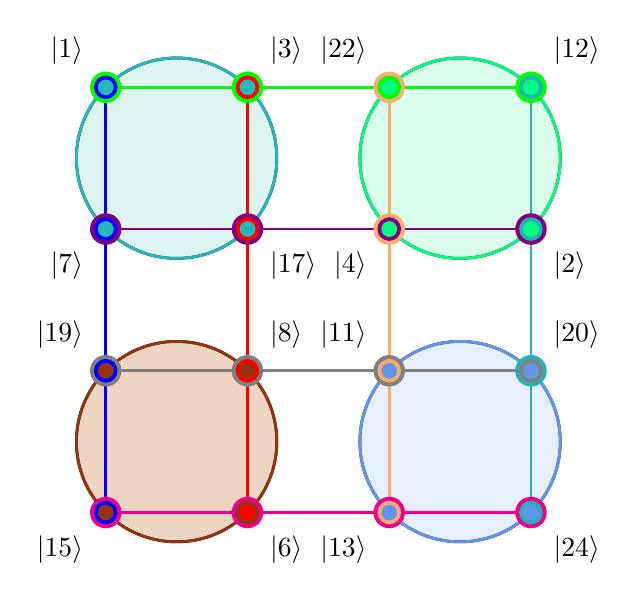
\begin{tikzpicture}  [scale=0.6]
\tikzstyle{every path}=[line width=1pt]   %,label distance=0.6pt
\newdimen\ms
\ms=0.1cm
        %\tikzstyle{c2}=[circle,inner sep=1pt,minimum size=5pt]
        %\tikzstyle{c1}=[circle,inner sep=0pt,minimum size=3pt]
\tikzstyle{c4}=[circle,inner sep={\ms/8},minimum size=5*\ms]
\tikzstyle{c3}=[circle,inner sep={\ms/8},minimum size=4*\ms]
\tikzstyle{c2}=[circle,inner sep={\ms/8},minimum size=3*\ms]
\tikzstyle{c1}=[circle,inner sep={\ms/8},minimum size=2*\ms]



        %%% Define positions of some observables
        \path
              (0,0) coordinate(1)
              (3,0) coordinate(2)
              (6,0) coordinate(3)
              (9,0) coordinate(4)
              (0,-3) coordinate(5)
              (3,-3) coordinate(6)
              (6,-3) coordinate(7)
              (9,-3) coordinate(8)
              (0,-6) coordinate(9)
              (3,-6) coordinate(10)
              (6,-6) coordinate(11)
              (9,-6) coordinate(12)
              (0,-9) coordinate(13)
              (3,-9) coordinate(14)
              (6,-9) coordinate(15)
              (9,-9) coordinate(16) ;




        %%% Draw all the context curves

       % small circles


\draw[fill=BlueGreen!15!white] (1.5,-1.5) circle (2.12132cm);
\draw[color=BlueGreen] (1.5,-1.5) circle (2.12132cm);

\draw[fill=SpringGreen!15!white] (7.5,-1.5) circle (2.12132cm);
\draw[color=SpringGreen] (7.5,-1.5) circle (2.12132cm);

\draw[fill=RawSienna!15!white] (1.5,-7.5) circle (2.12132cm);
\draw[color=RawSienna] (1.5,-7.5) circle (2.12132cm);

\draw[fill=CornflowerBlue!15!white] (7.5,-7.5) circle (2.12132cm);
\draw[color=CornflowerBlue] (7.5,-7.5) circle (2.12132cm);


        %  context liness horizontal

\draw [color=green] (1) -- (4);
\draw [color=violet] (5) -- (8);
\draw [color=gray] (9) -- (12);
\draw [color=magenta] (13) -- (16);

        %  context liness vertical

\draw [color=blue] (1) -- (13);
\draw [color=red] (2) -- (14);
\draw [color=Apricot] (3) -- (15);
\draw [color=TealBlue] (4) -- (16);




       % elements in context

\draw (1) coordinate[c3,fill=green,label=135:$\vert 1 \rangle$];
\draw (1) coordinate[c2,fill=blue];
\draw (1) coordinate[c1,fill=BlueGreen];

\draw (2) coordinate[c3,fill=green,label=45:$\vert 3 \rangle$];
\draw (2) coordinate[c2,fill=red];
\draw (2) coordinate[c1,fill=BlueGreen];

\draw (3) coordinate[c3,fill=Apricot,label=135:$\vert 22 \rangle$];
\draw (3) coordinate[c2,fill=green];
\draw (3) coordinate[c1,fill=SpringGreen];

\draw (4) coordinate[c3,fill=green,label=45:$\vert 12 \rangle$];
\draw (4) coordinate[c2,fill=TealBlue];
\draw (4) coordinate[c1,fill=SpringGreen];

\draw (5) coordinate[c3,fill=violet,label=225:$\vert 7 \rangle$];
\draw (5) coordinate[c2,fill=blue];
\draw (5) coordinate[c1,fill=BlueGreen];

\draw (6) coordinate[c3,fill=violet,label=-45:$\vert 17 \rangle$];
\draw (6) coordinate[c2,fill=red];
\draw (6) coordinate[c1,fill=BlueGreen];

\draw (7) coordinate[c3,fill=Apricot,label=-135:$\vert 4 \rangle$];
\draw (7) coordinate[c2,fill=violet];
\draw (7) coordinate[c1,fill=SpringGreen];

\draw (8) coordinate[c3,fill=violet,label=-45:$\vert 2 \rangle$];
\draw (8) coordinate[c2,fill=TealBlue];
\draw (8) coordinate[c1,fill=SpringGreen];

\draw (9) coordinate[c3,fill=gray,label=135:$\vert 19 \rangle$];
\draw (9) coordinate[c2,fill=blue];
\draw (9) coordinate[c1,fill=RawSienna];

\draw (10) coordinate[c3,fill=gray,label=45:$\vert 8 \rangle$];
\draw (10) coordinate[c2,fill=red];
\draw (10) coordinate[c1,fill=RawSienna];

\draw (11) coordinate[c3,fill=gray,label=135:$\vert 11\rangle$];
\draw (11) coordinate[c2,fill=Apricot];
\draw (11) coordinate[c1,fill=CornflowerBlue];

\draw (12) coordinate[c3,fill=TealBlue,label=45:$\vert 20 \rangle$];
\draw (12) coordinate[c2,fill=gray];
\draw (12) coordinate[c1,fill=CornflowerBlue];

\draw (13) coordinate[c3,fill=magenta,label=225:$\vert 15 \rangle$];
\draw (13) coordinate[c2,fill=blue];
\draw (13) coordinate[c1,fill=RawSienna];

\draw (14) coordinate[c3,fill=magenta,label=-45:$\vert 6 \rangle$];
\draw (14) coordinate[c2,fill=RawSienna];
\draw (14) coordinate[c1,fill=red];

\draw (15) coordinate[c3,fill=magenta,label=225:$\vert 13 \rangle$];
\draw (15) coordinate[c2,fill=Apricot];
\draw (15) coordinate[c1,fill=CornflowerBlue];

\draw (16) coordinate[c3,fill=magenta,label=-45:$\vert 24 \rangle$];
\draw (16) coordinate[c2,fill=TealBlue];
\draw (16) coordinate[c1,fill=CornflowerBlue];

    \end{tikzpicture}
}
    \end{minipage}%
&
    \begin{minipage}{0.27\textwidth}
\begin{tabular}{c}
\resizebox{1\textwidth}{!}{
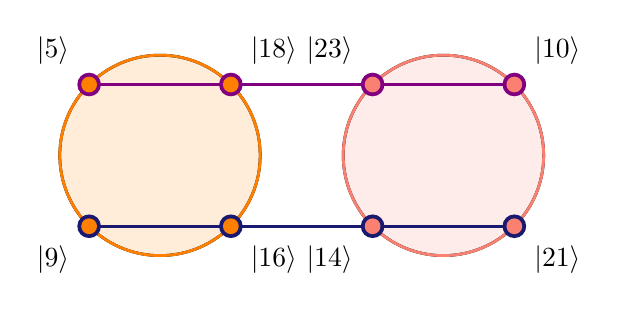
\begin{tikzpicture}  [scale=0.6]
\tikzstyle{every path}=[line width=1pt]   %,label distance=0.6pt
\newdimen\ms
\ms=0.1cm
        %\tikzstyle{c2}=[circle,inner sep=1pt,minimum size=5pt]
        %\tikzstyle{c1}=[circle,inner sep=0pt,minimum size=3pt]
\tikzstyle{c4}=[circle,inner sep={\ms/8},minimum size=5*\ms]
\tikzstyle{c3}=[circle,inner sep={\ms/8},minimum size=4*\ms]
\tikzstyle{c2}=[circle,inner sep={\ms/8},minimum size=3*\ms]
\tikzstyle{c1}=[circle,inner sep={\ms/8},minimum size=2*\ms]



        %%% Define positions of some observables
        \path
              (0,0) coordinate(1)
              (3,0) coordinate(2)
              (6,0) coordinate(3)
              (9,0) coordinate(4)
              (0,-3) coordinate(5)
              (3,-3) coordinate(6)
              (6,-3) coordinate(7)
              (9,-3) coordinate(8)
              ;




        %%% Draw all the context curves

       % small circles


\draw[fill=orange!15!white] (1.5,-1.5) circle (2.12132cm);
\draw[color=orange] (1.5,-1.5) circle (2.12132cm);

\draw[fill=Salmon!15!white] (7.5,-1.5) circle (2.12132cm);
\draw[color=Salmon] (7.5,-1.5) circle (2.12132cm);



        %  context liness horizontal

\draw [color=violet] (1) -- (4);
\draw [color=MidnightBlue] (5) -- (8);



       % elements in context

\draw (5) coordinate[c2,fill=MidnightBlue,label=225:$\vert 9 \rangle$];
\draw (5) coordinate[c1,fill=orange];

\draw (6) coordinate[c2,fill=MidnightBlue,label=-45:$\vert 16 \rangle$];
\draw (6) coordinate[c1,fill=orange];

\draw (8) coordinate[c2,fill=MidnightBlue,label=-45:$\vert 21 \rangle$];
\draw (8) coordinate[c1,fill=Salmon];

\draw (7) coordinate[c2,fill=MidnightBlue,label=225:$\vert 14 \rangle$];
\draw (7) coordinate[c1,fill=Salmon];

\draw (1) coordinate[c2,fill=violet,label=135:$\vert 5 \rangle$];
\draw (1) coordinate[c1,fill=orange];

\draw (2) coordinate[c2,fill=violet,label=45:$\vert 18 \rangle$];
\draw (2) coordinate[c1,fill=orange];

\draw (4) coordinate[c2,fill=violet,label=45:$\vert 10 \rangle$];
\draw (4) coordinate[c1,fill=Salmon];

\draw (3) coordinate[c2,fill=violet,label=135:$\vert 23 \rangle$];
\draw (3) coordinate[c1,fill=Salmon];


    \end{tikzpicture}
}
\\
\resizebox{1\textwidth}{!}{
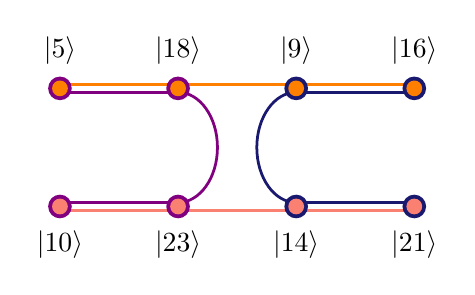
\begin{tikzpicture}  [scale=0.5]
\tikzstyle{every path}=[line width=1pt]   %,label distance=0.6pt
\newdimen\ms
\ms=0.1cm
        %\tikzstyle{c2}=[circle,inner sep=1pt,minimum size=5pt]
        %\tikzstyle{c1}=[circle,inner sep=0pt,minimum size=3pt]
\tikzstyle{c4}=[circle,inner sep={\ms/8},minimum size=5*\ms]
\tikzstyle{c3}=[circle,inner sep={\ms/8},minimum size=4*\ms]
\tikzstyle{c2}=[circle,inner sep={\ms/8},minimum size=3*\ms]
\tikzstyle{c1}=[circle,inner sep={\ms/8},minimum size=2*\ms]



        %%% Define positions of some observables
        \path
              (0,0.1) coordinate(1)
              (0,-0.1) coordinate(11)
              (0,0) coordinate(21)
              (3,0.1) coordinate(2)
              (3,-0.1) coordinate(12)
              (3,0) coordinate(22)
              (6,0.1) coordinate(5)
              (6,-0.1) coordinate(15)
              (6,0) coordinate(25)
              (9,0.1) coordinate(6)
              (9,-0.1) coordinate(16)
              (9,0) coordinate(26)
              (0,-3.1) coordinate(4)
              (0,-2.9) coordinate(14)
              (0,-3) coordinate(24)
              (3,-3.1) coordinate(3)
              (3,-2.9) coordinate(13)
              (3,-3) coordinate(23)
              (6,-3.1) coordinate(7)
              (6,-2.9) coordinate(17)
              (6,-3) coordinate(27)
              (9,-3.1) coordinate(8)
              (9,-2.9) coordinate(18)
              (9,-3) coordinate(28)
              ;




        %%% Draw all the context curves

       % small circles


%\draw[fill=orange!15!white] (1.5,-1.5) circle (2.12132cm);
%\draw[color=orange] (1.5,-1.5) circle (2.12132cm);

%\draw[fill=Salmon!15!white] (7.5,-1.5) circle (2.12132cm);
%\draw[color=Salmon] (7.5,-1.5) circle (2.12132cm);

%\node[ellipse, draw, color=BlueGreen, minimum width=1.3cm, minimum height=2.8cm] at (3,-1.5) {};

\draw [color=violet] (12) arc(90:-90:1cm and 1.4cm);
\draw [color=MidnightBlue] (15) arc(90:270:1cm and 1.4cm);

        %  context liness horizontal

\draw [color=orange] (1) -- (6);
\draw [color=violet] (11) -- (12);
\draw [color=MidnightBlue] (15) -- (16);
\draw [color=Salmon] (4) -- (8);
\draw [color=violet] (14) -- (13);
\draw [color=MidnightBlue] (17) -- (18);



       % elements in context

\draw (25) coordinate[c2,fill=MidnightBlue,label=90:$\vert 9 \rangle$];
\draw (25) coordinate[c1,fill=orange];

\draw (26) coordinate[c2,fill=MidnightBlue,label=90:$\vert 16 \rangle$];
\draw (26) coordinate[c1,fill=orange];

\draw (28) coordinate[c2,fill=MidnightBlue,label=-90:$\vert 21 \rangle$];
\draw (28) coordinate[c1,fill=Salmon];

\draw (27) coordinate[c2,fill=MidnightBlue,label=-90:$\vert 14 \rangle$];
\draw (27) coordinate[c1,fill=Salmon];

\draw (21) coordinate[c2,fill=violet,label=90:$\vert 5 \rangle$];
\draw (21) coordinate[c1,fill=orange];

\draw (22) coordinate[c2,fill=violet,label=90:$\vert 18 \rangle$];
\draw (22) coordinate[c1,fill=orange];

\draw (24) coordinate[c2,fill=violet,label=-90:$\vert 10 \rangle$];
\draw (24) coordinate[c1,fill=Salmon];

\draw (23) coordinate[c2,fill=violet,label=-90:$\vert 23 \rangle$];
\draw (23) coordinate[c1,fill=Salmon];


    \end{tikzpicture}
}
    \end{tabular}
    \end{minipage}%
\\
(a)&(b)&(c)
    \end{tabular}
\caption{\label{2024-convert-f-24-24}
(a)
Hypergraph representing contexts (or cliques or orthonormal bases or maximal operators) %enumerated in Table~\ref{2024-convert-matrixpencil-peres-DirectedLexOrdered-cliques}
as unbroken smooth lines. This is a `orthogonal completion'~\cite{peres-91,pavicic-2004ksafq} of the
KS set comprising 18 vectors in 9 contexts introduced by Cabello, Estebaranz and Garc{\'{i}}a-Alcaine~\cite{cabello-96}.
The filled shaded small ovals on the edges correspond to the `primary' isolated (nonintertwined) contexts from the matrix pencil calculations enumerated
in Table~\ref{2024-convert-matrixpencil-peres}.
(b)
Hypergraph representing a 16-12 configuration: 16 elements in 12 contexts enumerated in the first, second, fourth, and fifth row of Table~\ref{2024-convert-matrixpencil-peres}.
These vectors are separable and thus correspond to factorizable, nonentangled states.
(c)
Two equivalent hypergraph representations of a 8-4 configuration---8 elements in 4 contexts
enumerated in the third and sixth row of
Table~\ref{2024-convert-matrixpencil-peres}.
These vectors are nonseparable and thus correspond to entangled states.}
\end{figure*}




\section{Bipartite Greenberger-Horne-Zeilinger argument}


Based on the GHZ argument Mermin has suggested~\cite{mermin,mermin90b} a ``simple unified form for the major no-hidden-variables theorems'' in which he identified four commuting three-partite operators:
$\sigma_x \myotimes  \sigma_x \myotimes  \sigma_x$, $\sigma_x \myotimes  \sigma_y \myotimes  \sigma_y$, $\sigma_y \myotimes  \sigma_x \myotimes  \sigma_y$, and $\sigma_y \myotimes  \sigma_y \myotimes  \sigma_x$.
A parity argument reveals a state-independent quantum contradiction to the classical existence of (local, noncontextual) elements of physical reality:
The quantum mechanical expectation of the product of these four commuting three-partite operators for any quantum state is
$
-1= \langle
-\mathbb{1}_8
 \rangle
=
\langle
\mathbb{1}_2
\myotimes
(
-\mathbb{1}_2
)
\myotimes
\mathbb{1}_2
 \rangle
=
\langle
(
%\underbrace{
\sigma_x  \cdot \sigma_x  \cdot \sigma_y   \cdot \sigma_y
%}_{\mathbb{1}_2}
)
\myotimes
(
%\underbrace{
\sigma_x   \cdot \sigma_y   \cdot \sigma_x   \cdot  \sigma_y
%}_{-\mathbb{1}_2}
)
\myotimes
(
%\underbrace{
\sigma_x   \cdot \sigma_y    \cdot \sigma_y    \cdot \sigma_x
%}_{\mathbb{1}_2}
) \rangle
=
\langle  (\sigma_x \myotimes  \sigma_x \myotimes  \sigma_x) \cdot (\sigma_x \myotimes  \sigma_y \myotimes  \sigma_y) \cdot (\sigma_y \myotimes  \sigma_x \myotimes  \sigma_y) \cdot (\sigma_y \myotimes  \sigma_y \myotimes  \sigma_x) \rangle
=
\langle  \sigma_x \myotimes  \sigma_x \myotimes  \sigma_x  \rangle \langle \sigma_x \myotimes  \sigma_y \myotimes  \sigma_y  \rangle \langle
\sigma_y \myotimes  \sigma_x \myotimes  \sigma_y  \rangle \langle   \sigma_y \myotimes  \sigma_y \myotimes  \sigma_x \rangle
$.
In this formulation, every operator $\sigma_x$ and $\sigma_y$ for each of the three particles occurs twice. Therefore, if classically all such single-particle observables would coexist as elements of physical reality and independent of what other measurements are made alongside,
then their respective product must be $1$, the exact negative of the quantum expectation.


Mermin's configuration can be analyzed in terms of its matrix pencil
$
a \sigma_x \myotimes  \sigma_x \myotimes  \sigma_x + b \sigma_x \myotimes  \sigma_y \myotimes  \sigma_y + c \sigma_y \myotimes  \sigma_x \myotimes  \sigma_y + d \sigma_y \myotimes  \sigma_y \myotimes  \sigma_x
%\label{2024-convert-mpghzm}
$,
thereby revealing the underlying, hidden context in terms of
the simultaneous eigensystem of the four mutually commuting operators.
%
%enumerated in Table~\ref{2024-convert-mpghzm-es}.
%
%\begin{table*}[ht]
%\caption{\label{2024-convert-mpghzm-es}Eigensystem of the matrix pencil~\eqref{2024-convert-mpghzm}
%associated with the Mermin configuration~\cite{mermin,mermin90b}, constituting an orthogonal basis in an eight-dimensional Hilbert space.
%The values `$\boldsymbol{+}$' and `$\boldsymbol{-}$' represent the measured vales $+1$ and $-1$ of the respective operators.
%}
%\centering
%\begin{ruledtabular}
%\begin{tabular}{rlcccccccc}
% \multicolumn{1}{c}{eigenvalue} & \multicolumn{1}{c}{eigenvector} & $\sigma_x \myotimes  \sigma_x \myotimes  \sigma_x$ & $\sigma_x \myotimes  \sigma_y \myotimes  \sigma_y$ & $\sigma_x \myotimes  \sigma_y \myotimes  \sigma_y$ & $\sigma_y \myotimes  \sigma_y \myotimes  \sigma_x$ \\
%\hline
%   $-a + b - c - d $ &          $ \vert \Gamma_1 \rangle = \frac{1}{\sqrt{2}}\left( \vert z_+z_-z_- \rangle  - \vert z_-z_+z_+ \rangle \right) \equiv \begin{pmatrix}          0, 0, 0, 1, -1, 0, 0, 0            \end{pmatrix}^\intercal  $  &   $\boldsymbol{-}$ &  $\boldsymbol{+}$  & $\boldsymbol{-}$   & $\boldsymbol{-}$        \\
%   $a - b + c + d  $&           $ \vert \Gamma_2 \rangle = \frac{1}{\sqrt{2}}\left( \vert z_+z_-z_- \rangle  + \vert z_-z_+z_+ \rangle \right) \equiv \begin{pmatrix}          0, 0, 0, 1, 1, 0, 0, 0            \end{pmatrix}^\intercal   $  &   $\boldsymbol{+}$ &  $\boldsymbol{-}$  & $\boldsymbol{+}$   & $\boldsymbol{+}$       \\
%   $-a - b + c - d $ &          $ \vert \Gamma_3 \rangle = \frac{1}{\sqrt{2}}\left( \vert z_+z_-z_+ \rangle  - \vert z_-z_+z_- \rangle \right) \equiv \begin{pmatrix}          0, 0, 1, 0, 0, -1, 0, 0            \end{pmatrix}^\intercal  $  &   $\boldsymbol{-}$ &  $\boldsymbol{-}$  & $\boldsymbol{+}$   & $\boldsymbol{-}$        \\
%   $a + b - c + d  $&           $ \vert \Gamma_4 \rangle = \frac{1}{\sqrt{2}}\left( \vert z_+z_-z_+ \rangle  + \vert z_-z_+z_- \rangle \right) \equiv \begin{pmatrix}          0, 0, 1, 0, 0, 1, 0, 0            \end{pmatrix}^\intercal   $  &   $\boldsymbol{+}$ &  $\boldsymbol{+}$  & $\boldsymbol{-}$   & $\boldsymbol{+}$       \\
%   $-a - b - c + d $ &          $ \vert \Gamma_5 \rangle = \frac{1}{\sqrt{2}}\left( \vert z_+z_+z_- \rangle  - \vert z_-z_-z_+ \rangle \right) \equiv \begin{pmatrix}          0, 1, 0, 0, 0, 0, -1, 0            \end{pmatrix}^\intercal  $  &   $\boldsymbol{-}$ &  $\boldsymbol{-}$  & $\boldsymbol{-}$   & $\boldsymbol{+}$        \\
%   $  a + b + c - d$  &         $ \vert \Gamma_6 \rangle = \frac{1}{\sqrt{2}}\left( \vert z_+z_+z_- \rangle  + \vert z_-z_-z_+ \rangle \right) \equiv \begin{pmatrix}          0, 1, 0, 0, 0, 0,   1, 0            \end{pmatrix}^\intercal $  &   $\boldsymbol{+}$ &  $\boldsymbol{+}$  & $\boldsymbol{+}$   & $\boldsymbol{-}$         \\
%   $-a + b + c + d $&           $ \vert \Gamma_7 \rangle = \frac{1}{\sqrt{2}}\left( \vert z_+z_+z_+ \rangle  - \vert z_-z_-z_- \rangle \right) \equiv \begin{pmatrix}          1, 0, 0, 0, 0, 0, 0, -1            \end{pmatrix}^\intercal  $  &   $\boldsymbol{-}$ &  $\boldsymbol{+}$  & $\boldsymbol{+}$   & $\boldsymbol{+}$     \\
%   $a - b - c - d  $&           $ \vert \Gamma_8 \rangle = \frac{1}{\sqrt{2}}\left( \vert z_+z_+z_+ \rangle  + \vert z_-z_-z_- \rangle \right) \equiv \begin{pmatrix}          1, 0, 0, 0, 0, 0, 0, 1            \end{pmatrix}^\intercal   $  &   $\boldsymbol{+}$ &  $\boldsymbol{-}$  & $\boldsymbol{-}$   & $\boldsymbol{-}$       \\
%\end{tabular}
%\end{ruledtabular}
%\end{table*}
%
These eight nonseparable vectors form an orthonormal basis of an eight-dimensional Hilbert space corresponding to an isolated single context~\cite[Table~1]{svozil-2020-ghz} of  entangled states.
Therefore, Mermin's configuration does not constitute a KS proof, as it still permits a separating set of eight two-valued states.

In view of this, how does one arrive at a complete GHZ contradiction with classical elements of physical reality, as outlined above?
The criterion employed in an experimental corroboration~\cite{panbdwz} is to select any one of the eigenstates forming the orthonormal basis, such as
$
(1/\sqrt{2})
\big(
\vert z_+z_+z_+ \rangle  + \vert z_-z_-z_- \rangle
\big)
%= \begin{pmatrix}          1, 0, 0, 0, 0, 0, 0, 1            \end{pmatrix}^\intercal
$.
Since this is an eigenstate of all four terms of the matrix pencil, four separate measurements can be performed (possibly temporally separated) yielding the eigenvalues
$+1$ for
$\sigma_x \myotimes  \sigma_x \myotimes  \sigma_x$
as well as $-1$ for the three others. These three factors  $-1$ and one factor $+1$ contribute to their product value $-1$, in total contradiction to the classical expectation $+1$.
Note that similar contradictions arise if the seven other eigenstates of the matrix pencil are considered~\cite[Table~1]{svozil-2020-ghz}.
%These quantum-versus-classical discrepancies are independent of the specific state.
%We chose the particular state $\vert \Gamma_8 \rangle$ because it is---among the eight eigenstates enumerated in Table~\ref{2024-convert-mpghzm-es}---an eigenstate of the individual terms involved in the matrix pencil.


%As we have seen, the quantum logic and hypergraph representation of the GHZ-Mermin argument is basic---indeed, it amounts to a single context hypergraph representable by a line~\cite[Figure~2(a)]{svozil-2020-ghz}.
%The `strength' of its conviction lies in its operational realizability as a collection of four, preferably nonlocal
%(under strict Einstein separability) measurements of the operators mentioned, and applied to one of the eigenstates~\cite{panbdwz}.
%Since all the operators involved mutually commute, they could theoretically be serially composed--applied one after the other in any order.
%%However, such a scenario would undermine the nonlocality, as it would require the respective input and output ports to be aligned.

Can an equally convincing argument be made for just two particles?
Natural candidates would be the `nonclassical' elements of the PM square~\eqref{2024-convert-PeresSquare}.
Note that its `masked' or `hidden' contexts, revealed by the matrix pencils, can be partitioned into four `separable' type contexts
depicted in Figure~\ref{2024-convert-f-24-24}(b)
containing only separable vectors---corresponding to the first and second rows and columns---and two `nonclassical' contexts consisting of nonseparable
vectors---corresponding to the last row and column, as depicted in
Figure~\ref{2024-convert-f-24-24}(c).
%Those latter observables the four-dimensional equivalent
%of the (v-shaped) `firefly logic'~\cite[pp. 21-22]{cohen} in three dimensions
%with dichotomic degenerate operators taking on the role of quantum logical propositions:
%the `intertwining' observable $\sigma_y \myotimes \sigma_y$ `connects' two contexts,
%namely the one formed by
%$\{ \sigma_x \myotimes \sigma_z , \sigma_y \myotimes \sigma_y , \sigma_z \myotimes \sigma_x\}$,
%and
%$\{ \sigma_x \myotimes \sigma_x, \sigma_y \myotimes \sigma_y, \sigma_z \myotimes \sigma_z\}$.



Concentrating on these two latter contexts consisting of nonseparable vectors, we make the following observations:
%(i)
Since the observables from the last row and last column (with the exception of  $\sigma_y \myotimes \sigma_y$) do not commute, they cannot be simultaneously measured.
%(ii)
Nevertheless, by forming products within the last row and column, we may create two commuting operators
%in classical terms, the same `elements of physical reality', namely
%$(\sigma_z \myotimes \sigma_x) \cdot (\sigma_x \myotimes \sigma_z) \cdot (\sigma_y \myotimes \sigma_y)$
%and
%$(\sigma_z \myotimes \sigma_z) \cdot (\sigma_x \myotimes \sigma_x) \cdot (\sigma_y \myotimes \sigma_y)$.
%Within the contexts, that is, if they belong to the same product, any of these factors can be simultaneously measured.
%And yet, quantum mechanically, the first product yields $\mathbb{1}_4$ and the second $-\mathbb{1}_4$,
%and thus their respective expectations (on any state) are $+1$ and $-1$ This latter prediction is in total contradiction with classical expectations.
%
%The product of these two products contains an even number of classical supposedly `elements of physical reality' for both particles,
%similarly to the GHZ-Mermin argument for three particles.
%Dissimilar to the latter  it involves two contexts rather than just one.
%One may object that the two-partite `analog' is trivial in the sense that one effectively `merely measures identities' and not the individual expectations.
%This is due to complementarity, as, say,  $\sigma_x \myotimes \sigma_x$ is not in the same context as $\sigma_x \myotimes \sigma_z$.
%But it should be kept in mind that the basic presumptions remain the same in both arguments.
%
%The argument could be made shorter and possibly more convincing by realizing that the following operators commute because of equality:
$
(\sigma_z \myotimes \sigma_x) \cdot (\sigma_x \myotimes \sigma_z) = -(\sigma_x \myotimes \sigma_x) \cdot (\sigma_z \myotimes \sigma_z)
=
(\sigma_z \cdot \sigma_x ) \myotimes (\sigma_x \cdot \sigma_z)
=   \sigma_y  \myotimes \sigma_y
= \text{antidiag}
\begin{pmatrix} -1 , 1 ,1, -1
\end{pmatrix}
$.
%They share the Bell basis as common system of eigenvectors.
Their matrix pencil
\begin{equation}
%\begin{split}
a(\sigma_z \myotimes \sigma_x) \cdot (\sigma_x \myotimes \sigma_z) + b (\sigma_x \myotimes \sigma_x) \cdot (\sigma_z \myotimes \sigma_z)
% + c (\sigma_y \myotimes \sigma_y) \cdot (\sigma_y \myotimes \sigma_y)
%\end{split}
\label{2024-convert-mppm}
\end{equation}
has a degenerate spectrum with the Bell basis as eigenvectors---the same as the eigenvectors of the matrix pencil of the last column of the PM square. It is enumerated in Table~\ref{2024-convert-pm-es}.


Hence, preparing a state in one Bell basis state and measuring (successively or separately)
$
(\sigma_z \myotimes \sigma_x) \cdot (\sigma_x \myotimes \sigma_z)
$,
and
$
(\sigma_x \myotimes \sigma_x) \cdot (\sigma_z \myotimes \sigma_z)
$
or
$
\sigma_x \myotimes \sigma_x
$
as well as
$
\sigma_z \myotimes \sigma_z
$ separately,
yields
\begin{equation}
\begin{split}  -1 =
\langle
-\mathbb{1}_4
 \rangle
=
\langle
\mathbb{1}_2 \myotimes (-\mathbb{1}_2)
 \rangle
\\
=
 \langle
(\sigma_z  \cdot \sigma_x \cdot \sigma_x \cdot \sigma_z ) \myotimes (\sigma_x \cdot \sigma_z \cdot  \sigma_x \cdot \sigma_z)
 \rangle
\\
=
\langle
(\sigma_z \myotimes \sigma_x) \cdot (\sigma_x \myotimes \sigma_z)   \cdot
(\sigma_x \myotimes \sigma_x) \cdot (\sigma_z \myotimes \sigma_z)
\rangle
\\
=
\langle
(\sigma_z \myotimes \sigma_x) \cdot (\sigma_x \myotimes \sigma_z)\rangle
\langle  (\sigma_x \myotimes \sigma_x) \cdot (\sigma_z \myotimes \sigma_z) \rangle
.
\end{split}
\end{equation}

In contrast, and in analogy to Mermin's version of the GHZ argument, the classical prediction is that the product of these terms always needs to be positive, as every alleged `element of reality', in particular corresponding to $\sigma_x$ and $\sigma_z$, enters an even number of times (indeed, twice per particle).



\begin{table}[t]
\caption{\label{2024-convert-pm-es}Eigensystem of the matrix pencil~\eqref{2024-convert-mppm}
associated with the commuting  products of operators in the last (third) row and the last (third) column of the PM square,
constituting the Bell basis.
Inclusion of  $(\sigma_y \myotimes \sigma_y) \cdot (\sigma_y \myotimes \sigma_y) = \mathbb{1}_4$
does not change the calculation and is therefore omitted.
The values $+1$ and $-1$ represent the (co)measured values of the respective commuting operators.
}
\centering
\begin{ruledtabular}
\begin{tabular}{rccccccccc}
\multicolumn{1}{c}{value} &
\multicolumn{1}{c}{vector} &
$(\sigma_z \myotimes  \sigma_x) \cdot (\sigma_x\myotimes  \sigma_z)$ &
$\sigma_x \myotimes  \sigma_x$ &
$\sigma_z\myotimes  \sigma_z$ &
$(\sigma_x \myotimes  \sigma_x) \cdot  (\sigma_z\myotimes  \sigma_z)$
\\
\hline
   $a - b$ &          $ \vert \Psi_+ \rangle $   &   $+1$  &  $+1$    &  $-1$   &  $-1$      \\
   $a - b$ &          $ \vert \Phi_- \rangle $   &   $+1$  &  $-1$    &  $+1$   &  $-1$      \\
   $-a + b$ &         $ \vert \Psi_- \rangle $   &   $-1$  &  $-1$    &  $-1$   &  $+1$      \\
   $-a + b$ &         $ \vert \Phi_+ \rangle $   &   $-1$  &  $+1$    &  $+1$   &  $+1$      \\
\end{tabular}
\end{ruledtabular}
\end{table}


I conclude with some comments and an outlook.
A nonlocal measurement in quantum mechanics refers to the simultaneous measurement of properties of entangled particles that are---at least in principle---located in space-like separated regions (Einstein locality).
We therefore suggest calling an operator, or a collection of mutually commuting operators, `nonlocal' if they---or more generally, the eigensystem of their matrix pencil---allow entangled, that is, nonseparable, eigenstates after projective measurements.
This is the case for the last row and column of the PM square, and also for the four three-partite operators suggested by Mermin in the context of the GHZ argument.
I shall motivate and discuss these issues further in a later publication.

%We have concentrated on transcriptions of operator-based arguments against the classical performance of quantized systems with dichotomic arguments.
%These methods allow the generalization to non-dichotomic outcomes.
%A converse transcription in terms of a hypergraph representing (possibly intertwining) contexts into nonlocal measurements can be achieved if this hypergraph allows a faithful orthogonal representation~\cite{lovasz-79,Portillo-2015}
%(or, equivalently, a coordinatization~\cite{Pavii2018}) in terms of vector labels that are entangled (or, equivalently, nonfactorizable).
%
%The sum of noncommuting operators such as the Clauser-Horne-Shimony-Holt operator
%$
%\sigma_1 \myotimes \sigma_3
%+
%\sigma_1 \myotimes \sigma_4
%+
%\sigma_2 \myotimes \sigma_3
%-
%\sigma_2 \myotimes \sigma_4
%$
%with
%$\sigma_i= \sigma ( \theta_i ,\varphi_i )$
%can be analized by acknowledging that the sum of products of scalars with normal operators is also a normal operator.
%Therefore, this sum has a (not necessarily unique if the sum is degenerate)
%spectral decomposition in terms of projection operators corresponding to some orthonormal basis.
%This orthonormal basis forms an isolated context whose elements may be simultaneously measured
%and optimized~\cite{filipp-svo-04-qpoly-prl}.
%Alternatively, the contexts formed by the spectral decompositions of the individual summands can be considered as the basis of the analysis.

The matrix pencil method provides an elegant solution for simultaneously diagonalizing commuting operators with degenerate spectra.
It offers a systematic approach for the application of `contextual' nonclassical performance in quantized systems, particularly in delineating operator-valued arguments.

The PM square demonstrates a fundamental contradiction (quantum $-1$ versus classical $+1$) compared to classical existence in a dichotomic operator-valued formulation.
By employing matrix pencils, this contradiction can be transcribed into a KS type argument with 24 vectors.
This configuration,
which does not support any  binary (two-valued) state,
consist of 6 `original' isolated contexts from the matrix pencils associated with every row and column of the PM square, as well as 18 `secondary' intertwining contexts obtained by studying orthogonalities.

Mermin's rendition of the GHZ operator-valued argument is indeed altogether different.
When transcribed into quantum logic, it reveals a single isolated context that is perfectly set representable, for instance, by partition logic.
Thereby, the quantum state becomes crucial for any experimental corroboration:
if one takes any eigenstate of the matrix pencil it leads to a complete contradiction  (again quantum $-1$ versus classical $+1$)
when multiplying all the results and comparing the squares of operators in a parity argument.


In analyzing the `entangled contexts' corresponding to the last row and column of the PM square and
constructing mutually commuting products thereof, one arrives at a very similar argument as Mermin's rendition of the GHZ argument.
It is also state-independent and operates within a single context. The operators are:
$
(\sigma_z \myotimes \sigma_x) \cdot (\sigma_x \myotimes \sigma_z)
$  and alternatively,
$
(\sigma_x\myotimes \sigma_x) \cdot (\sigma_z\myotimes \sigma_z)
$
or
$
\sigma_x\myotimes \sigma_x
$
and
$\sigma_z\myotimes \sigma_z
$
and, although not needed for the constraction,
$(\sigma_y \myotimes \sigma_y) \cdot (\sigma_y\myotimes \sigma_y)$.
These operators commute, and for the Bell basis yield at a complete contradiction
(quantum $-1$ versus classical $+1$) contingent on the assumption of noncontextual classical existence
of those elements of physical reality.
This reduces the eight-dimensional argument to a four-dimensional one.
It might be interesting to probe the factors
$
\sigma_z \cdot \sigma_x
$
and
$\sigma_x\cdot \sigma_z
$
of the tensor product
$
(\sigma_z \myotimes \sigma_x) \cdot (\sigma_x \myotimes \sigma_z)
= (\sigma_z \cdot \sigma_x) \myotimes (\sigma_x \cdot \sigma_z)
$
by the Bell states
$|\Psi_-\rangle$
and
$|\Phi_+\rangle$
in an Einstein-Podolsky-Rosen configuration,
because this alone could `isolate' the `rub', as the quantum prediction of the observed value would be
$-1$.
Likewise,
application of the  Bell states
$|\Psi_+\rangle$
and
$|\Phi_-\rangle$
on
$
(\sigma_z \myotimes \sigma_z) \cdot (\sigma_x \myotimes \sigma_x)
= (\sigma_z \cdot \sigma_x) \myotimes (\sigma_z \cdot \sigma_x)
$
would result in an observed value $-1$.


Why or how can such operator-valued contradictions arise in the context of a single isolated context?
Because measurements like $\sigma_x \myotimes \sigma_y ( \myotimes \sigma_y)$ as part of a context from a matrix pencil should not be perceived as `local'
and cannot be performed as two (or three) single-qubit
local measurements~\cite{cabello2021contextuality}.
Such operator-valued arguments are based on a classically justified conviction that every two- (or three-) particle state can be composed of single-particle states  in such a way that the former retains all properties of the latter.
This is no longer true for entangled states, which encode relational information at the (unitary) cost of
abandonment of local properties.
From this perspective, both dichotomic operator-valued GHZ arguments as well as binary two-valued state KS arguments against noncontextuality
share a nonoperational and thus (meta)physical presumption: the contingent use of counterfactuals.


\begin{acknowledgments}

This research was funded in whole or in part by the Austrian Science Fund (FWF), Grant-DOI: 10.55776/I4579. For open access purposes, the author has applied a CC BY public copyright license to any author accepted manuscript version arising from this submission.

A question by Bruno Mittnik stimulated this research.
I acknowledge explanations from Costantino Budroni, Ad\'an Cabello and Jan-\AA{}ke Larsson regarding aspects of Reference~\cite{cabello2021contextuality},
as well as explanations, discussions, and suggestions from Mladen Pavicic regarding the properties of the 24-24 configuration.
(Any remaining confusion remains solely with the author.)
%The author declares no conflict of interest.
\end{acknowledgments}



\bibliography{svozil}
\bibliographystyle{apsrev}



\end{document}




%%%%%%%%%%%%%%%%%%%%%%%%%%%%%%%%%%%%%%%%%%%%%%%%%%%%%%%%%%%%%%%%%%%%%%%%%%%%%%%%%%%%%%%%%%%%%%%%%%%%%%%%%%%%
%%%%%%%%%%%%%%%%%%%%%%%%%%%%%%%%%%%%%%%%%%%%%%%%%%%%%%%%%%%%%%%%%%%%%%%%%%%%%%%%%%%%%%%%%%%%%%%%%%%%%%%%%%%%
%%%%%%%%%%%%%%%%%%%%%%%%%%%%%%%%%%%%%%%%%%%%%%%%%%%%%%%%%%%%%%%%%%%%%%%%%%%%%%%%%%%%%%%%%%%%%%%%%%%%%%%%%%%%
%%%%%%%%%%%%%%%%%%%%%%%%%%%%%%%%%%%%%%%%%%%%%%%%%%%%%%%%%%%%%%%%%%%%%%%%%%%%%%%%%%%%%%%%%%%%%%%%%%%%%%%%%%%%
%%%%%%%%%%%%%%%%%%%%%%%%%%%%%%%%%%%%%%%%%%%%%%%%%%%%%%%%%%%%%%%%%%%%%%%%%%%%%%%%%%%%%%%%%%%%%%%%%%%%%%%%%%%%
%%%%%%%%%%%%%%%%%%%%%%%%%%%%%%%%%%%%%%%%%%%%%%%%%%%%%%%%%%%%%%%%%%%%%%%%%%%%%%%%%%%%%%%%%%%%%%%%%%%%%%%%%%%%
%%%%%%%%%%%%%%%%%%%%%%%%%%%%%%%%%%%%%%%%%%%%%%%%%%%%%%%%%%%%%%%%%%%%%%%%%%%%%%%%%%%%%%%%%%%%%%%%%%%%%%%%%%%%


From the matrix pencil operations it can be deduced that
measurements of each observable in the
last row and last column of the PM square~(\ref{2024-convert-PeresSquare}) cannot be performed as two single-qubit
local measurements: compare, for instance, the system of eigenvectors of the matrix pencil
$
a \sigma_z  \myotimes   \sigma_x + b \sigma_x  \myotimes   \sigma_z + c \sigma_y  \myotimes   \sigma_y
$.
These eigenvectors
(cf. third matrix pencil of Table~\ref{2024-convert-matrixpencil-peres})
belong to entangled (indecomposable)  states, as the product of their outer coordinates is the negative of (and thus unqual to)
the products of their inner coordinates.
A more detailed analysis shows that the plane, say, spanned by the eigenvectors
with degenerate eigenvalues for $a=1$ and $b=c=0$,
$ \begin{pmatrix}  1, 1, -1, 1\end{pmatrix}^\intercal $ and  $ \begin{pmatrix}  1, 1, 1, -1\end{pmatrix}^\intercal $ carries a continuum of pure entangled (indecomposable) states,
with the exception of two onedimensional subspaces spanned by
$ \begin{pmatrix}  1, 1, -1, 1\end{pmatrix}^\intercal  \pm   \begin{pmatrix}  1, 1, 1, -1\end{pmatrix}^\intercal $~\cite{havlicek-svozil-2020-dec}.
In any case, a projection operator formed by the dyadic product of (normalized) indecomposable eigenvectors cannot correspond to a two single-qubit local measurement.


Indeed, except for singular parameter choices of measure zero,
even measurements of the general form   $\sigma ( \theta_1 ,\varphi_1 ) \myotimes  \sigma ( \theta_2 ,\varphi_2 )$, have eigenvalues
$  \{  -1 , -1 , 1 , 1\} $ and associated eigenvectors
\begin{equation}
\begin{aligned}
&  \begin{pmatrix}  -e^{-i (\phi_1+\phi_2)}   \sin \theta_2 ,e^{-i \phi_1}  (\cos \theta_1+\cos \theta_2) ,0,\sin \theta_1 \end{pmatrix}^\intercal         ,
\\
&  \begin{pmatrix}  e^{-i   \phi_1}  (\cos \theta_1-\cos   \theta_2) ,-e^{-i (\phi_1-\phi_2)}    \sin \theta_2 ,\sin \theta_1,0  \end{pmatrix}^\intercal    ,
\\
&   \begin{pmatrix}  e^{-i  (\phi_1+\phi_2)}  \sin \theta_2 ,e^{-i  \phi_1} (\cos \theta_1-\cos  \theta_2) ,0,\sin \theta_1 \end{pmatrix}^\intercal       ,
\\
&  \begin{pmatrix}  e^{-i \phi_1}  (\cos \theta_1+\cos \theta_2) ,e^{-i   (\phi_1-\phi_2)}  \sin   \theta_2 ,\sin \theta_1,0  \end{pmatrix}^\intercal     ,
\end{aligned}
\label{2024-convert-esgtqlm}
\end{equation}
with a vanishing coordinate equal to $0$, and thus correspond to entangled states
(with the exception of $\theta_1=0$ or $\theta_2=0$ and $\phi_1=\phi_2=0$).


%%%%%%%%%%%%%%%%%%%%%%%%%%%%%%%%%%%%%%%%%%%%%%%%%%%%%%%%%%%%%%%%%%%%%%%%%%%%%%%%%%%%%%%%%%%%%%%%%%%%%%%%%%%%
%%%%%%%%%%%%%%%%%%%%%%%%%%%%%%%%%%%%%%%%%%%%%%%%%%%%%%%%%%%%%%%%%%%%%%%%%%%%%%%%%%%%%%%%%%%%%%%%%%%%%%%%%%%%
%%%%%%%%%%%%%%%%%%%%%%%%%%%%%%%%%%%%%%%%%%%%%%%%%%%%%%%%%%%%%%%%%%%%%%%%%%%%%%%%%%%%%%%%%%%%%%%%%%%%%%%%%%%%

WRONG:

In this line of argument we may employ the matrix pencil of the last (third) column of the PM square~(\ref{2024-convert-PeresSquare}), and confront it with
the Bell basis vector $\vert \Phi_+ \rangle =   (1/\sqrt{2})\big( \vert HH \rangle +  \vert VV \rangle \big) = \begin{pmatrix}          1, 0, 0, 1            \end{pmatrix}^\intercal $.
Because by the parity argument, classically, every observable in this column occurs twice, so multiplication results in squares of the observed vales.
As those are real, this product should classically result in a nonnegative number.
however, the eigenvalues of $\vert \Psi_+ \rangle$ are $+1$ for
$\sigma_x \myotimes  \sigma_x$   and $\sigma_z \myotimes  \sigma_z$ but $-1$ for $\sigma_y \myotimes  \sigma_y$.
When measuring them in the same way (possibly successively and temporally separated one after the other), this product
$
\langle (\sigma_x \myotimes  \sigma_x) \cdot (\sigma_z \myotimes  \sigma_z) \cdot (\sigma_y \myotimes  \sigma_y) \rangle
=\langle (\sigma_x \myotimes  \sigma_x) \rangle \langle (\sigma_z \myotimes  \sigma_z)  \rangle \langle (\sigma_y \myotimes  \sigma_y) \rangle
= -1$
is negative.
Thus, Mermin's two-partite transcription of the KS paradox appears to be as `nonclassical' as the GHZ argument, relative to the assumptions and means of the latter~\cite{panbdwz}.
Note that also in this case any one of the four eigenvectors---the vectors in the Bell basis, in particular, also the singlet state---resulting from the matrix pencil calculation, suffices for an non-probabilistic argument against classicality.



In this line of argument, we may utilize the matrix pencil of the last (third) column of the PM square~(\ref{2024-convert-PeresSquare}),
and compare it with the Bell basis vector $\vert \Phi_+ \rangle = (1/\sqrt{2})\left( \vert HH \rangle + \vert VV \rangle \right) = \begin{pmatrix} 1 , 0 , 0 , 1 \end{pmatrix}^\intercal $.
By the parity argument, classically, every observable in this column occurs twice, resulting in squares of the observed values.
Since these values are real, this product should classically yield a nonnegative number.
However, the eigenvalues of $\vert \Psi_+ \rangle$ are $+1$ for $\sigma_x \myotimes  \sigma_x$ and $\sigma_z \myotimes  \sigma_z$, but $-1$ for $\sigma_y \myotimes  \sigma_y$.
When measuring them in the same way (possibly successively and temporally separated),
the product $\langle (\sigma_x \myotimes  \sigma_x) \cdot (\sigma_z \myotimes  \sigma_z) \cdot (\sigma_y \myotimes  \sigma_y) \rangle = -1$ is negative.
From this point of view, Mermin's two-partite transcription of the KS paradox appears to be as `nonclassical' as the GHZ argument,
relative to the assumptions and means of the latter~\cite{panbdwz}.

Note that in this case, any one of the four eigenvectors resulting from the matrix pencil calculation---the vectors in the Bell basis, in particular, also the singlet state---suffices for a non-probabilistic
GHZ type argument against classicality.
This, of course, begs the immediate question: if the same can be achieved with classical shares such as Peres' exploding bomb~\cite{peres222}---in what way is this form of quantum contextuality different from, say, KS type configurations?
Because whereas the quantum performance of the full PM square cannot be classically emulated, a singly isolated context can.

%%%%%%%%%%%%%%%%%%%%%%%%%%%%%%%%%%%%%%%%%%%%%%%%%%%%%%%%%%%%%%%%%%%%%%%%%%%%%%%%%%%%%%%%%%%%%%%%%%%%%%%%%%%%
%%%%%%%%%%%%%%%%%%%%%%%%%%%%%%%%%%%%%%%%%%%%%%%%%%%%%%%%%%%%%%%%%%%%%%%%%%%%%%%%%%%%%%%%%%%%%%%%%%%%%%%%%%%%
%%%%%%%%%%%%%%%%%%%%%%%%%%%%%%%%%%%%%%%%%%%%%%%%%%%%%%%%%%%%%%%%%%%%%%%%%%%%%%%%%%%%%%%%%%%%%%%%%%%%%%%%%%%%
%%%%%%%%%%%%%%%%%%%%%%%%%%%%%%%%%%%%%%%%%%%%%%%%%%%%%%%%%%%%%%%%%%%%%%%%%%%%%%%%%%%%%%%%%%%%%%%%%%%%%%%%%%%%
%%%%%%%%%%%%%%%%%%%%%%%%%%%%%%%%%%%%%%%%%%%%%%%%%%%%%%%%%%%%%%%%%%%%%%%%%%%%%%%%%%%%%%%%%%%%%%%%%%%%%%%%%%%%
%%%%%%%%%%%%%%%%%%%%%%%%%%%%%%%%%%%%%%%%%%%%%%%%%%%%%%%%%%%%%%%%%%%%%%%%%%%%%%%%%%%%%%%%%%%%%%%%%%%%%%%%%%%%
%%%%%%%%%%%%%%%%%%%%%%%%%%%%%%%%%%%%%%%%%%%%%%%%%%%%%%%%%%%%%%%%%%%%%%%%%%%%%%%%%%%%%%%%%%%%%%%%%%%%%%%%%%%%
%%%%%%%%%%%%%%%%%%%%%%%%%%%%%%%%%%%%%%%%%%%%%%%%%%%%%%%%%%%%%%%%%%%%%%%%%%%%%%%%%%%%%%%%%%%%%%%%%%%%%%%%%%%%



(*Question:

What contexts are "hiding beneath" the 3rd row of Equation \
(5) of

@article{cabello2021contextuality,author={Costantino Budroni \
and Ad\'an Cabello and Otfried G\"uhne and Matthias Kleinmann and \
Jan-\AA{}ke \
Larsson},eprint={arXiv:2102.13036},url={https://https://doi.org/10.\
1103/RevModPhys.94.045007},doi={10.1103/revmodphys.94.045007},year=\
2022,month={dec},publisher={American Physical Society \
({APS})},volume={94},number={4},title={{K}ochen-{S}pecker \
contextuality},journal={Reviews of Modern \
Physics},pages={045007}}?*)


(*Definition of "my" Tensor Product*)(*a,b are nxn and mxm-matrices*)

MyTensorProduct[a_, b_] :=
  Table[a[[Ceiling[s/Length[b]], Ceiling[t/Length[b]]]]*
    b[[s - Floor[(s - 1)/Length[b]]*Length[b],
      t - Floor[(t - 1)/Length[b]]*Length[b]]], {s, 1,
    Length[a]*Length[b]}, {t, 1, Length[a]*Length[b]}];

(*Definition of the Dyadic Product*)

DyadicProductVec[x_] :=
  Table[x[[i]]  Conjugate[x[[j]]], {i, 1, Length[x]}, {j, 1,
    Length[x]}];

(*Commutator*)

Commutator[a_, b_] := a . b - b . a;


(*************************************************************************************)

yJ = MyTensorProduct[PauliMatrix[2], IdentityMatrix[2]];
Jy = MyTensorProduct[IdentityMatrix[2], PauliMatrix[2]];
yx = MyTensorProduct[PauliMatrix[2], PauliMatrix[1]];
xy = MyTensorProduct[PauliMatrix[1], PauliMatrix[2]];


zJ = MyTensorProduct[PauliMatrix[3], IdentityMatrix[2]];
Jz = MyTensorProduct[IdentityMatrix[2], PauliMatrix[3]];
zz = MyTensorProduct[PauliMatrix[3], PauliMatrix[3]];

Jx = MyTensorProduct[IdentityMatrix[2], PauliMatrix[1]];
xJ = MyTensorProduct[PauliMatrix[1], IdentityMatrix[2]];
xx = MyTensorProduct[PauliMatrix[1], PauliMatrix[1]];

zx = MyTensorProduct[PauliMatrix[3], PauliMatrix[1]];
xz = MyTensorProduct[PauliMatrix[1], PauliMatrix[3]];
yy = MyTensorProduct[PauliMatrix[2], PauliMatrix[2]];


(*

Print["Commutators"]


Commutator[zx, xz]
Commutator[zx, yy]
Commutator[xz, yy]


MatrixForm[Commutator[zJ, zx]]

*)

Print["Eigensystem by matrix pencil calculation"]

Eigensystem[a   zJ + b   Jz + c   zz]

Eigensystem[a   Jx + b   xJ + c   xx]

Eigensystem[a   zx + b   xz + c   yy]

Eigensystem[a   zJ + b   Jx + c   zx]

Eigensystem[a   Jz + b   xJ + c   xz]

Eigensystem[a   zz + b   xx + c   yy]



union = Union[Eigenvectors[a    zJ + b    Jz + c    zz],
  Eigenvectors[a    Jx + b    xJ + c    xx],
  Eigenvectors[a    zx + b    xz + c    yy],
  Eigenvectors[a    zJ + b    Jx + c    zx],
  Eigenvectors[a    Jz + b    xJ + c    xz],
  Eigenvectors[a    zz + b    xx + c    yy]]


(*

uniondirected =
  Table[If[union[[i, 1]] < 0, -union[[i]], union[[i]]], {i, 1,
    Length[union]}];

udir = Union[uniondirected]

Length[udir]

*)

ulexsorted=
{
{0, 0, 0, 1},
{0, 0, 1, -1},
{0, 0, 1,  0},
{0, 0, 1, 1},
{0, 1, -1, 0},
{0, 1, 0, -1},
{0, 1, 0, 0},
{0, 1, 0, 1},
{0, 1, 1,  0},
{1, -1, -1, -1},
{1, -1, -1, 1},
{1, -1, 0, 0},
{1, -1,  1, -1},
{1, -1, 1, 1},
{1, 0, -1, 0},
{1, 0, 0, -1},
{1, 0, 0,  0},
{1, 0, 0, 1},
{1, 0, 1, 0},
{1, 1, -1, -1},
{1, 1, -1, 1},
{1,   1, 0, 0},
{1, 1, 1, -1},
{1, 1, 1, 1}
};

LexicographicSort[{
{0, 0, 0, 1},
{0, 0, 1, -1},
{0, 0, 1,  0},
{0, 0, 1, 1},
{0, 1, -1, 0},
{0, 1, 0, -1},
{0, 1, 0, 0},
{0, 1, 0, 1},
{0, 1, 1,  0},
{1, -1, -1, -1},
{1, -1, -1, 1},
{1, -1, 0, 0},
{1, -1,  1, -1},
{1, -1, 1, 1},
{1, 0, -1, 0},
{1, 0, 0, -1},
{1, 0, 0,  0},
{1, 0, 0, 1},
{1, 0, 1, 0},
{1, 1, -1, -1},
{1, 1, -1, 1},
{1,   1, 0, 0},
{1, 1, 1, -1},
{1, 1, 1, 1}
}  ] === {
{0, 0, 0, 1},
{0, 0, 1, -1},
{0, 0, 1,  0},
{0, 0, 1, 1},
{0, 1, -1, 0},
{0, 1, 0, -1},
{0, 1, 0, 0},
{0, 1, 0, 1},
{0, 1, 1,  0},
{1, -1, -1, -1},
{1, -1, -1, 1},
{1, -1, 0, 0},
{1, -1,  1, -1},
{1, -1, 1, 1},
{1, 0, -1, 0},
{1, 0, 0, -1},
{1, 0, 0,  0},
{1, 0, 0, 1},
{1, 0, 1, 0},
{1, 1, -1, -1},
{1, 1, -1, 1},
{1,   1, 0, 0},
{1, 1, 1, -1},
{1, 1, 1, 1}
}

OrthogonalityMatrix =
  Table[If[FullSimplify[ulexsorted[[i]] . ulexsorted[[j]]] == 0, 1, 0]
        , {i,Length[ulexsorted]}, {j, Length[ulexsorted]}];

MatrixForm[OrthogonalityMatrix];

g = AdjacencyGraph[OrthogonalityMatrix];

FindClique[g, {1}, 100]

FindClique[g, {2}, 100]

FindClique[g, {3}, 100]

FindClique[g, {4}, 100]

FindClique[g, {5}, 100]


%%%%%%%%%%%%%%%%%%%%%%%%%%%%%%%%%%%%%%%%%%%%%%%%%%%%%%%%%%%%%%%%%%%%%%%%%%%%%%%%%%%%%%%%%%%%%%%%%%%%%%%%%%

Extended 18-9 set
24 atoms
24 blocks
 0 proper subsets of blocks
 4   5  9 16 18
 4   3  7 16 18
 4   9 14 16 21
 4   9 13 18 20
 4  11 13 20 24
 4   5 11 16 24
 4  10 14 21 23
 4   5 10 18 23
 4   8 14 15 23
 4   8 11 19 20
 4   6 13 15 24
 4   6 10 19 21
 4   6  8 15 19
 4   3  6  8 17
 4   4 12 21 23
 4   4 11 13 22
 4   2 12 20 24
 4   2 10 14 22
 4   2  4 12 22
 4   2  4  7 17
 4   1  7 15 19
 4   1  5  9 17
 4   1  3 12 22
 4   1  3  7 17
0 2-valued evaluations of atoms:

set of 2-valued evaluations of atoms:
nonempty: no



%%%%%%%%%%%%%%%%%%%%%%%%%%%%%%%%%%%%%%%%%%%%%%%%%%%%%%%%%%%%%%%%%%%%%%%%%%%%%%%%%%%%%%%%%%%%%%%%%%%%%%


(* GHZ-Stairs-Mermin configuration *)




(*Definition of "my" Tensor Product*)(*a,b are nxn and mxm-matrices*)

MyTensorProduct[a_, b_] :=
  Table[a[[Ceiling[s/Length[b]], Ceiling[t/Length[b]]]]*
    b[[s - Floor[(s - 1)/Length[b]]*Length[b],
      t - Floor[(t - 1)/Length[b]]*Length[b]]], {s, 1,
    Length[a]*Length[b]}, {t, 1, Length[a]*Length[b]}];

(*Definition of the Dyadic Product*)

DyadicProductVec[x_] :=
  Table[x[[i]]  Conjugate[x[[j]]], {i, 1, Length[x]}, {j, 1,
    Length[x]}];

(*Commutator*)

Commutator[a_, b_] := a . b - b . a;


(* *********************************




a xxx + b yyx + c yxy + d xyy
a y11 + b yyx + c 11x + d 1y1
a y11 + b yxy + c 11y + d 1x1
a xxx + b 11x + c x11 + d 1x1
a xyy + b 11y + c x11 + d 1y1


*)






yJJ = MyTensorProduct[MyTensorProduct[PauliMatrix[2], IdentityMatrix[2]],IdentityMatrix[2]];
xxx = MyTensorProduct[MyTensorProduct[PauliMatrix[1], PauliMatrix[1]],PauliMatrix[1]];
yyx = MyTensorProduct[MyTensorProduct[PauliMatrix[2], PauliMatrix[2]],PauliMatrix[1]];
yxy = MyTensorProduct[MyTensorProduct[PauliMatrix[2], PauliMatrix[1]],PauliMatrix[2]];
xyy = MyTensorProduct[MyTensorProduct[PauliMatrix[1], PauliMatrix[2]],PauliMatrix[2]];
JJx = MyTensorProduct[MyTensorProduct[IdentityMatrix[2], IdentityMatrix[2]],PauliMatrix[1]];
JJy = MyTensorProduct[MyTensorProduct[IdentityMatrix[2], IdentityMatrix[2]], PauliMatrix[2]];
xJJ = MyTensorProduct[MyTensorProduct[PauliMatrix[1], IdentityMatrix[2]], IdentityMatrix[2]];
JyJ = MyTensorProduct[MyTensorProduct[IdentityMatrix[2], PauliMatrix[2]], IdentityMatrix[2]];
JxJ = MyTensorProduct[MyTensorProduct[IdentityMatrix[2],PauliMatrix[1]], IdentityMatrix[2]];

Eigensystem[a xxx + b yyx + c yxy + d xyy  ]

Eigensystem[a yJJ + b yyx + c JJx + d JyJ  ]

Eigensystem[a yJJ + b yxy + c JJy + d JxJ  ]

Eigensystem[a xxx + b JJx + c xJJ + d JxJ  ]

Eigensystem[a xyy + b JJy + c xJJ + d JyJ  ]



union = Union[Eigenvectors[a xxx + b yyx + c yxy + d xyy  ],
      Eigenvectors[a yJJ + b yyx + c JJx + d JyJ  ],
      Eigenvectors[a yJJ + b yxy + c JJy + d JxJ  ],
      Eigenvectors[a xxx + b JJx + c xJJ + d JxJ  ],
      Eigenvectors[a xyy + b JJy + c xJJ + d JyJ  ]
];

uniondirected = Table[ If[ union[[i,1]] < 0, -union[[i]], union[[i]] ]
,{i, 1,Length[union]}];

udir= Union[uniondirected]

Length[udir]

OrthogonalityMatrix =
 Table[ If[ FullSimplify[udir[[i]] . udir[[j]]] == 0, 1, 0]
  , {i, Length[udir]}, {j, Length[udir]}];

MatrixForm[ OrthogonalityMatrix ]

g = AdjacencyGraph[OrthogonalityMatrix]

FindClique[g, {2}, 100]

FindClique[g, {3}, 100]

FindClique[g, {4}, 100]

FindClique[g, {5}, 100]

FindClique[g, {6}, 100]

FindClique[g, {7}, 100]

FindClique[g, {8}, 100]

FindClique[g, {9}, 100]

FindClique[g, {10}, 100]


%%%%%%%%%%%%%%%%%%%%%%%%%%%%%%%%%%%%%%%%%%%%%%%%%%%%%%%%%%%%%%%%%%%%%%%%%%%%%%%%%%%%%%%%%%%%%%%%%%%%%

(* GHZ--Shimony-Mermin configuration *)




(*Definition of "my" Tensor Product*)(*a,b are nxn and mxm-matrices*)

MyTensorProduct[a_, b_] :=
  Table[a[[Ceiling[s/Length[b]], Ceiling[t/Length[b]]]]*
    b[[s - Floor[(s - 1)/Length[b]]*Length[b],
      t - Floor[(t - 1)/Length[b]]*Length[b]]], {s, 1,
    Length[a]*Length[b]}, {t, 1, Length[a]*Length[b]}];

(*Definition of the Dyadic Product*)

DyadicProductVec[x_] :=
  Table[x[[i]]  Conjugate[x[[j]]], {i, 1, Length[x]}, {j, 1,
    Length[x]}];

(*Commutator*)

Commutator[a_, b_] := a . b - b . a;


(* *********************************

 Mermin GHZ


a xxx + b xyy + c yxy + d yyx



*)






yJJ = MyTensorProduct[MyTensorProduct[PauliMatrix[2], IdentityMatrix[2]],IdentityMatrix[2]];
xxx = MyTensorProduct[MyTensorProduct[PauliMatrix[1], PauliMatrix[1]],PauliMatrix[1]];
yyx = MyTensorProduct[MyTensorProduct[PauliMatrix[2], PauliMatrix[2]],PauliMatrix[1]];
yxy = MyTensorProduct[MyTensorProduct[PauliMatrix[2], PauliMatrix[1]],PauliMatrix[2]];
xyy = MyTensorProduct[MyTensorProduct[PauliMatrix[1], PauliMatrix[2]],PauliMatrix[2]];
JJx = MyTensorProduct[MyTensorProduct[IdentityMatrix[2], IdentityMatrix[2]],PauliMatrix[1]];
JJy = MyTensorProduct[MyTensorProduct[IdentityMatrix[2], IdentityMatrix[2]], PauliMatrix[2]];
xJJ = MyTensorProduct[MyTensorProduct[PauliMatrix[1], IdentityMatrix[2]], IdentityMatrix[2]];
JyJ = MyTensorProduct[MyTensorProduct[IdentityMatrix[2], PauliMatrix[2]], IdentityMatrix[2]];
JxJ = MyTensorProduct[MyTensorProduct[IdentityMatrix[2],PauliMatrix[1]], IdentityMatrix[2]];


MatrixForm[FullSimplify[xxx . xyy . yxy . yyx]]


xyy . yxy . yyx == -xxx


Eigensystem[a xxx + b xyy + c yxy + d yyx  ]




union = Union[Eigenvectors[a xxx + b xyy + c yxy + d yyx  ]
];

uniondirected = Table[ If[ union[[i,1]] < 0, -union[[i]], union[[i]] ]
,{i, 1,Length[union]}];

udir= Union[uniondirected]

Length[udir]

OrthogonalityMatrix =
 Table[ If[ FullSimplify[udir[[i]] . udir[[j]]] == 0, 1, 0]
  , {i, Length[udir]}, {j, Length[udir]}];

MatrixForm[ OrthogonalityMatrix ]

g = AdjacencyGraph[OrthogonalityMatrix]

FindClique[g, {8}, 100]



%%%%%%%%%%%%%%%%%%%%%%%%%%%%%%%%%%%%%%%%%%%%%%%%%%%%%%%%%%%%%%%%%%%%%%%%%%%%%%%%%%%%%%%%%%%%%%%%%%%%%%%%%
union={{0,0,0,1},
{0,0,1,0},
{1,1,0,0},
{1,-1,0,0},
{1,0,0,0},
{0,1,0,0},
{0,0,1,-1},
{0,0,1,1},
{0,1,-1,0},
{1,0,0,1},
{-1,1,1,1},
{1,1,1,-1},
{0,1,1,0},
{1,0,0,-1},
{1,-1,1,1},
{1,1,-1,1}
};

uniondirected = Table[ If[ union[[i,1]] < 0, -union[[i]], union[[i]] ]
,{i, 1,Length[union]}];

udir= uniondirected

Length[udir]

OrthogonalityMatrix =
 Table[ If[ FullSimplify[udir[[i]] . udir[[j]]] == 0, 1, 0]
  , {i, Length[udir]}, {j, Length[udir]}];

MatrixForm[ OrthogonalityMatrix ]

g = AdjacencyGraph[OrthogonalityMatrix]

FindClique[g, {2}, 100]

FindClique[g, {3}, 100]

FindClique[g, {4}, 100]

FindClique[g, {5}, 100]

FindClique[g, {6}, 100]

FindClique[g, {7}, 100]

FindClique[g, {8}, 100]

FindClique[g, {9}, 100]

FindClique[g, {10}, 100]

%%%%%%%%%%%%%%%%%%%%%%%%%%%%%%%%%%%%%%%%%%%%%%%%%%%%%%%%%%%%%%%%%%%%%%%%%%%%%%%%%%%%%%%%%%%%%%%%%%%%%%%%%%
%%%%%%%%%%%%%%%%%%%%%%%%%%%%%%%%%%%%%%%%%%%%%%%%%%%%%%%%%%%%%%%%%%%%%%%%%%%%%%%%%%%%%%%%%%%%%%%%%%%%%%%%%%

unitaryma =  (1/(2*Sqrt[2])) FullSimplify[
TensorProduct[   Transpose[{1, 1, -1, 1     }], {0, 1, 0, 1 }  ]+
TensorProduct[   Transpose[{1, -1, 1, 1     }], {-1, 0, 1, 0}  ]+
TensorProduct[   Transpose[{-1, 1, 1,  1    }], {0, -1, 0, 1}  ]+
TensorProduct[   Transpose[{-1, -1, -1, 1   }], {1, 0, 1,  0}  ] ]

MatrixForm[unitaryma]


(* check unitary? *)

unitaryma . Transpose[unitaryma] ==   IdentityMatrix[4]

(* check rotation? *)

unitaryma. Transpose[(1/Sqrt[2]){0, 1, 0, 1 }] == (1/2) {1, 1, -1, 1     }



Eigensystem[ PauliMatrix[3] ]         (* {{-1, 1}, {{0, 1}, {1, 0}}} *)

Eigensystem[ PauliMatrix[1] ]         (* {{-1, 1}, {{-1, 1}, {1, 1}}} *)


zzxx =  Flatten[TensorProduct[   {0, 1}, {-1, 1} ]] +  Flatten[TensorProduct[   {1, 0}, Transpose [{1, 1}] ]] -
           (Flatten[TensorProduct[   {0, 1}, {1, 1} ]] +  Flatten[TensorProduct[   {1, 0}, Transpose [{-1, 1}] ]])


zx = MyTensorProduct[PauliMatrix[3], PauliMatrix[1]];

unitaryma . zx . Transpose[unitaryma]

Eigensystem[unitaryma . zx . Transpose[unitaryma]]


%%%%%%%%%%%%%%%%%%%%%%%%%%%%%%%%%%%%%%%%%%%%%%%%%%%%%%%%%%%%%%%%%%%%%%%%

(*Definition of "my" Tensor Product*)(*a,b are nxn and mxm-matrices*)

MyTensorProduct[a_, b_] :=
  Table[a[[Ceiling[s/Length[b]], Ceiling[t/Length[b]]]]*
    b[[s - Floor[(s - 1)/Length[b]]*Length[b],
      t - Floor[(t - 1)/Length[b]]*Length[b]]], {s, 1,
    Length[a]*Length[b]}, {t, 1, Length[a]*Length[b]}];

(*Definition of the Dyadic Product*)

DyadicProductVec[x_] :=
  Table[x[[i]]  Conjugate[x[[j]]], {i, 1, Length[x]}, {j, 1,
    Length[x]}];

(*Commutator*)

Commutator[a_, b_] := a . b - b . a;


(*************************************************************************************)

yJ = MyTensorProduct[PauliMatrix[2], IdentityMatrix[2]];
Jy = MyTensorProduct[IdentityMatrix[2], PauliMatrix[2]];
yx = MyTensorProduct[PauliMatrix[2], PauliMatrix[1]];
xy = MyTensorProduct[PauliMatrix[1], PauliMatrix[2]];


zJ = MyTensorProduct[PauliMatrix[3], IdentityMatrix[2]];
Jz = MyTensorProduct[IdentityMatrix[2], PauliMatrix[3]];
zz = MyTensorProduct[PauliMatrix[3], PauliMatrix[3]];

Jx = MyTensorProduct[IdentityMatrix[2], PauliMatrix[1]];
xJ = MyTensorProduct[PauliMatrix[1], IdentityMatrix[2]];
xx = MyTensorProduct[PauliMatrix[1], PauliMatrix[1]];

zx = MyTensorProduct[PauliMatrix[3], PauliMatrix[1]];
xz = MyTensorProduct[PauliMatrix[1], PauliMatrix[3]];
yy = MyTensorProduct[PauliMatrix[2], PauliMatrix[2]];




Print["Eigensystem by matrix pencil calculation"]



avzxxzyy = Eigenvectors[a   zx + b   xz + c   yy]

sigma[t_,p_] := {{ Cos[t], E^(-I * p) Sin[t] },{ E^(I * p) Sin[t], -Cos[ t] }};


aevg =FullSimplify[ Eigenvectors[ MyTensorProduct[sigma[t1,p1], sigma[t2,p2]] ]]


##########################################################################

upo = Union[Permutations[{1, 1, 0, 0, 0, 0, 0, 0}],
 Permutations[{1, -1, 0, 0, 0, 0, 0, 0}],
 Permutations[{1, 1, 1, 1, 0, 0, 0, 0}],
 Permutations[{1, 1, -1, -1, 0, 0, 0, 0}],
 Permutations[{1, 1, 1, -1, 0, 0, 0, 0}],
 Permutations[{1, 1, 1, 1, 1, 1, 0, 0}],
 Permutations[{1, 1, 1, -1, -1, -1, 0, 0}],
 Permutations[{1, 1, 1, 1, -1, -1, 0, 0}],
 Permutations[{1, 1, 1, 1, 1, -1, 0, 0}],
 Permutations[{1, 1, 1, 1, 1, 1, 1, 1}],
 Permutations[{1, 1, 1, 1, -1, -1, -1, -1}],
 Permutations[{1, 1, 1, 1, 1, -1, -1, -1}],
 Permutations[{1, 1, 1, 1, 1, 1, -1, -1}],
 Permutations[{1, 1, 1, 1, 1, 1, 1, -1}]
 ]

Length[upo]



uniondirected = Table[
If[ upo[[i,1]] < 0, -upo[[i]], upo[[i]] ]
,{i, 1,Length[upo]}];

uniondirected1 = Table[
If[ (upo[[i,2]] < 0) && (upo[[i,1]] == 0), -uniondirected[[i]], uniondirected[[i]] ]
,{i, 1,Length[upo]}];

uniondirected =  uniondirected1;

uniondirected1 = Table[
If[ (upo[[i,3]] < 0) && (upo[[i,1]] == 0) && (upo[[i,2]] == 0), -uniondirected[[i]], uniondirected[[i]] ]
,{i, 1,Length[upo]}];

uniondirected =  uniondirected1;

uniondirected1 = Table[
If[ (upo[[i,4]] < 0) && (upo[[i,1]] == 0) && (upo[[i,2]] == 0)&& (upo[[i,3]] == 0), -uniondirected[[i]], uniondirected[[i]] ]
,{i, 1,Length[upo]}];

uniondirected =  uniondirected1;

uniondirected1 = Table[
If[ (upo[[i,5]] < 0) && (upo[[i,1]] == 0) && (upo[[i,2]] == 0)&& (upo[[i,3]] == 0) && (upo[[i,4]] == 0), -uniondirected[[i]], uniondirected[[i]] ]
,{i, 1,Length[upo]}];


uniondirected =  uniondirected1;

uniondirected1 = Table[
If[ (upo[[i,6]] < 0) && (upo[[i,1]] == 0) && (upo[[i,2]] == 0)&& (upo[[i,3]] == 0) && (upo[[i,4]] == 0) && (upo[[i,5]]== 0),-uniondirected[[i]], uniondirected[[i]] ]
,{i, 1,Length[upo]}];


uniondirected =  uniondirected1;

uniondirected1 = Table[
If[ (upo[[i,7]] < 0) && (upo[[i,1]] == 0) && (upo[[i,2]] == 0)&& (upo[[i,3]] == 0) && (upo[[i,4]] == 0) && (upo[[i,5]]== 0) && (upo[[i,6]]== 0),-uniondirected[[i]], uniondirected[[i]] ]
,{i, 1,Length[upo]}];


up= Union[uniondirected1];

Length[up]

OrthogonalityMatrix =
 Table[ If[ FullSimplify[up[[i]] . up[[j]]] == 0, 1, 0]
  , {i, Length[up]}, {j, Length[up]}];


g = AdjacencyGraph[OrthogonalityMatrix]

(* FindClique[g, {2}, 100]

FindClique[g, {3}, 100]

FindClique[g, {4}, 100]

FindClique[g, {5}, 100]

FindClique[g, {6}, 100]

FindClique[g, {7}, 100]
*)

FindClique[g, {8}, 100]



%%%%%%%%%%%%%%%%%%%%%%%%%%%%%%%%%%%%%%%%%%%%%%%%%%%%%%%%%%%%%%%%%%%%%%%%%%%%%%%%%%%%%%%%%%%


(*Definition of "my" Tensor Product*)(*a,b are nxn and mxm-matrices*)

MyTensorProduct[a_, b_] :=
  Table[a[[Ceiling[s/Length[b]], Ceiling[t/Length[b]]]]*
    b[[s - Floor[(s - 1)/Length[b]]*Length[b],
      t - Floor[(t - 1)/Length[b]]*Length[b]]], {s, 1,
    Length[a]*Length[b]}, {t, 1, Length[a]*Length[b]}];

(*Definition of the Dyadic Product*)

DyadicProductVec[x_] :=
  Table[x[[i]]  Conjugate[x[[j]]], {i, 1, Length[x]}, {j, 1,
    Length[x]}];

(*Commutator*)

Commutator[a_, b_] := a . b - b . a;


(* *********************************

 Mermin GHZ


a xxx + b xyy + c yxy + d yyx



*)






yJJ = MyTensorProduct[MyTensorProduct[PauliMatrix[2], IdentityMatrix[2]],IdentityMatrix[2]];
xxx = MyTensorProduct[MyTensorProduct[PauliMatrix[1], PauliMatrix[1]],PauliMatrix[1]];
yyx = MyTensorProduct[MyTensorProduct[PauliMatrix[2], PauliMatrix[2]],PauliMatrix[1]];
yxy = MyTensorProduct[MyTensorProduct[PauliMatrix[2], PauliMatrix[1]],PauliMatrix[2]];
xyy = MyTensorProduct[MyTensorProduct[PauliMatrix[1], PauliMatrix[2]],PauliMatrix[2]];
JJx = MyTensorProduct[MyTensorProduct[IdentityMatrix[2], IdentityMatrix[2]],PauliMatrix[1]];
JJy = MyTensorProduct[MyTensorProduct[IdentityMatrix[2], IdentityMatrix[2]], PauliMatrix[2]];
xJJ = MyTensorProduct[MyTensorProduct[PauliMatrix[1], IdentityMatrix[2]], IdentityMatrix[2]];
JyJ = MyTensorProduct[MyTensorProduct[IdentityMatrix[2], PauliMatrix[2]], IdentityMatrix[2]];
JxJ = MyTensorProduct[MyTensorProduct[IdentityMatrix[2],PauliMatrix[1]], IdentityMatrix[2]];


MatrixForm[FullSimplify[xxx . xyy . yxy . yyx]]


xyy . yxy . yyx == -xxx


%%%%%%%%%%%%%%%%%%%%%%%%%%%%%%%%%%%%%%%%%%%%%%%%%%%%%%%%%%%%%%%%%%%%%%%%%%%%%%%%%%%%%%%%%%



(*Definition of "my" Tensor Product*)(*a,b are nxn and mxm-matrices*)

MyTensorProduct[a_, b_] :=
  Table[a[[Ceiling[s/Length[b]], Ceiling[t/Length[b]]]]*
    b[[s - Floor[(s - 1)/Length[b]]*Length[b],
      t - Floor[(t - 1)/Length[b]]*Length[b]]], {s, 1,
    Length[a]*Length[b]}, {t, 1, Length[a]*Length[b]}];

(*Definition of the Dyadic Product*)

DyadicProductVec[x_] :=
  Table[x[[i]]  Conjugate[x[[j]]], {i, 1, Length[x]}, {j, 1,
    Length[x]}];

(*Commutator*)

Commutator[a_, b_] := a . b - b . a;


(*************************************************************************************)

yJ = MyTensorProduct[PauliMatrix[2], IdentityMatrix[2]];
Jy = MyTensorProduct[IdentityMatrix[2], PauliMatrix[2]];
yx = MyTensorProduct[PauliMatrix[2], PauliMatrix[1]];
xy = MyTensorProduct[PauliMatrix[1], PauliMatrix[2]];


zJ = MyTensorProduct[PauliMatrix[3], IdentityMatrix[2]];
Jz = MyTensorProduct[IdentityMatrix[2], PauliMatrix[3]];
zz = MyTensorProduct[PauliMatrix[3], PauliMatrix[3]];

Jx = MyTensorProduct[IdentityMatrix[2], PauliMatrix[1]];
xJ = MyTensorProduct[PauliMatrix[1], IdentityMatrix[2]];
xx = MyTensorProduct[PauliMatrix[1], PauliMatrix[1]];

zx = MyTensorProduct[PauliMatrix[3], PauliMatrix[1]];
xz = MyTensorProduct[PauliMatrix[1], PauliMatrix[3]];
yy = MyTensorProduct[PauliMatrix[2], PauliMatrix[2]];



Print["Eigensystem by matrix pencil calculation"]

Eigensystem[a   zx + b   xz + c   yy]


Eigensystem[a   zz + b   xx + c   yy]



union = Union[
  Eigenvectors[a    zx + b    xz + c    yy],
  Eigenvectors[a    zz + b    xx + c    yy]]




uniondirected =
  Table[If[union[[i, 1]] < 0, -union[[i]], union[[i]] ], {i, 1,
    Length[union]}];

udir = Union[uniondirected]

Length[udir]


OrthogonalityMatrix =
  Table[If[udir[[i]] . udir[[j]] == 0, 1, 0]
        , {i,Length[udir]}, {j, Length[udir]}];

MatrixForm[OrthogonalityMatrix];

g = AdjacencyGraph[OrthogonalityMatrix];

FindClique[g, {1}, 100]

FindClique[g, {2}, 100]

FindClique[g, {3}, 100]

FindClique[g, {4}, 100]

FindClique[g, {5}, 100]

%%%%%%%%%%%%%%%%%%%%%%%%%%%%%%%%%%%%%%%%%%%%%%%%%%%%%%%%%%%%%%%%%%%%%%%%%%%%%%%%%%%%
%%%%%%%%%%%%%%%%%%%%%%%%%%%%%%%%%%%%%%%%%%%%%%%%%%%%%%%%%%%%%%%%%%%%%%%%%%%%%%%%%%%%
%%%%%%%%%%%%%%%%%%%%%%%%%%%%%%%%%%%%%%%%%%%%%%%%%%%%%%%%%%%%%%%%%%%%%%%%%%%%%%%%%%%%
%%%%%%%%%%%%%%%%%%%%%%%%%%%%%%%%%%%%%%%%%%%%%%%%%%%%%%%%%%%%%%%%%%%%%%%%%%%%%%%%%%%%
%%%%%%%%%%%%%%%%%%%%%%%%%%%%%%%%%%%%%%%%%%%%%%%%%%%%%%%%%%%%%%%%%%%%%%%%%%%%%%%%%%%%


(*Definition of "my" Tensor Product*)(*a,b are nxn and mxm-matrices*)

MyTensorProduct[a_, b_] :=
  Table[a[[Ceiling[s/Length[b]], Ceiling[t/Length[b]]]]*
    b[[s - Floor[(s - 1)/Length[b]]*Length[b],
      t - Floor[(t - 1)/Length[b]]*Length[b]]], {s, 1,
    Length[a]*Length[b]}, {t, 1, Length[a]*Length[b]}];

(*Definition of the Dyadic Product*)

DyadicProductVec[x_] :=
  Table[x[[i]]  Conjugate[x[[j]]], {i, 1, Length[x]}, {j, 1,
    Length[x]}];

(*Commutator*)

Commutator[a_, b_] := a . b - b . a;


(*************************************************************************************)

yJ = MyTensorProduct[PauliMatrix[2], IdentityMatrix[2]];
Jy = MyTensorProduct[IdentityMatrix[2], PauliMatrix[2]];
yx = MyTensorProduct[PauliMatrix[2], PauliMatrix[1]];
xy = MyTensorProduct[PauliMatrix[1], PauliMatrix[2]];


zJ = MyTensorProduct[PauliMatrix[3], IdentityMatrix[2]];
Jz = MyTensorProduct[IdentityMatrix[2], PauliMatrix[3]];
zz = MyTensorProduct[PauliMatrix[3], PauliMatrix[3]];

Jx = MyTensorProduct[IdentityMatrix[2], PauliMatrix[1]];
xJ = MyTensorProduct[PauliMatrix[1], IdentityMatrix[2]];
xx = MyTensorProduct[PauliMatrix[1], PauliMatrix[1]];

zx = MyTensorProduct[PauliMatrix[3], PauliMatrix[1]];
xz = MyTensorProduct[PauliMatrix[1], PauliMatrix[3]];
yy = MyTensorProduct[PauliMatrix[2], PauliMatrix[2]];




bbpsip ={0,1,1,0};
bbpsim ={0,1,-1,0};
bbphip ={1,0,0,1};
bbphim ={1,0,0,-1};

ta=
{
{
zx.xz .    bbpsip,
xx.zz .    bbpsip,
yy.yy .    bbpsip
},
{
zx.xz .    bbpsim,
xx.zz .    bbpsim ,
yy.yy .    bbpsim
},
{
zx.xz .    bbphip ,
xx.zz .    bbphip   ,
yy.yy .    bbphip
},
{
zx.xz .    bbphim    ,
xx.zz .    bbphim     ,
yy.yy .    bbphim
}
}

MatrixForm[ta]

Eigensystem[a zx.xz +b xx.zz +c yy.yy]

##################################################################################################


(*Definition of "my" Tensor Product*)(*a,b are nxn and mxm-matrices*)
MyTensorProduct[a_, b_] :=
  Table[a[[Ceiling[s/Length[b]], Ceiling[t/Length[b]]]]*
    b[[s - Floor[(s - 1)/Length[b]]*Length[b],
      t - Floor[(t - 1)/Length[b]]*Length[b]]], {s, 1,
    Length[a]*Length[b]}, {t, 1, Length[a]*Length[b]}];

(*Definition of the Dyadic Product*)

DyadicProductVec[x_] :=
  Table[x[[i]]   Conjugate[x[[j]]], {i, 1, Length[x]}, {j, 1,
    Length[x]}];

(*Commutator*)

Commutator[a_, b_] := a . b - b . a;


(*************************************************************************************)

yJ = MyTensorProduct[PauliMatrix[2], IdentityMatrix[2]];
Jy = MyTensorProduct[IdentityMatrix[2], PauliMatrix[2]];
yx = MyTensorProduct[PauliMatrix[2], PauliMatrix[1]];
xy = MyTensorProduct[PauliMatrix[1], PauliMatrix[2]];


zJ = MyTensorProduct[PauliMatrix[3], IdentityMatrix[2]];
Jz = MyTensorProduct[IdentityMatrix[2], PauliMatrix[3]];
zz = MyTensorProduct[PauliMatrix[3], PauliMatrix[3]];

Jx = MyTensorProduct[IdentityMatrix[2], PauliMatrix[1]];
xJ = MyTensorProduct[PauliMatrix[1], IdentityMatrix[2]];
xx = MyTensorProduct[PauliMatrix[1], PauliMatrix[1]];

zx = MyTensorProduct[PauliMatrix[3], PauliMatrix[1]];
xz = MyTensorProduct[PauliMatrix[1], PauliMatrix[3]];
yy = MyTensorProduct[PauliMatrix[2], PauliMatrix[2]];



psim = {0, 1, -1, 0};
psip = {0, 1, +1, 0};
phim = {1, 0, 0, -1};
phip = {1, 0, 0, +1};


MatrixForm[ {
{xx.zz.psim ,  xx.psim ,  zz.psim ,  yy.psim },
{xx.zz.psip ,  xx.psip ,  zz.psip ,  yy.psip },
{xx.zz.phim ,  xx.phim ,  zz.phim ,  yy.phim },
{xx.zz.phip ,  xx.phip ,  zz.phip ,  yy.phip }}]
